\documentclass{article}
\usepackage[utf8]{inputenc}
\usepackage[a4paper]{geometry}
\usepackage{multicol}
\usepackage{graphicx}
\usepackage[round]{natbib}
\usepackage{amsmath}
\usepackage{framed}
\usepackage{palatino}
\usepackage[absolute]{textpos}
\usepackage{xcolor}
\usepackage{setspace}
\usepackage{float}
\usepackage[nottoc,numbib]{tocbibind}
\usepackage{tabularx}
\usepackage{lscape}
\usepackage{mdframed}
\usepackage{hologo}
\usepackage{rotating}
\usepackage{verbatim}
\usepackage{xcolor}
\usepackage[section]{placeins}
\usepackage{tikz}
\usepackage{tikzpeople}
\usepackage[toc,numberedsection=autolabel]{glossaries}
\graphicspath{{images/pdf/}}
\usetikzlibrary{shapes}
\tikzset{>=Latex}
\usepackage[pdfusetitle, pdfkeywords={Autonomous Vehicles, Risk Management, Cybersecurity},]{hyperref}
\usepackage{lettrine}
\usepackage{ltablex}
\definecolor{UniversitaetFarbe}{RGB}{0,101,189}
\doublespacing
\newtheorem{assumption}{Assumption}


%\def \pwd {/Users/david/Desktop/David_Bailey_Thesis}
%\newcommand{\executeiffilenewer}[3]{\ifnum\pdfstrcmp{\pdffilemoddate{#1}}{\pdffilemoddate{#2}}>0{#3}\fi}
%\newcommand{\dottopdf}[1]{\immediate\write18{dot -Tsvg \pwd/images/dot/#1.dot -o \pwd/images/svg/#1.svg}\immediate\write18{inkscape -D -z --file=\pwd/images/svg/#1.svg --export-pdf=\pwd/images/pdf/#1.pdf --export-latex}}
%\newcommand{\includedot}[1]{\executeiffilenewer{\pwd/images/dot/#1.dot}{\pwd/images/pdf/#1.pdf}{\dottopdf{#1}}\input{images/pdf/#1.pdf_tex}}
% add "shell_escape_commands = inkscape,dot" to /usr/local/texlive/2016/texmf.cnf

\makeglossaries
\newglossaryentry{defense in depth}{name=defense in depth, description={the use of multiple layers of security controls to protect a system while allowing for failures of individual controls}}
\newglossaryentry{confidentiality, integrity, and availability}{name={confidentiality, integrity, and availability}, description={the three pillars of information security}}
\newglossaryentry{confidentiality}{name=confidentiality, description={protecting information from theft, one of the three pillars of information security}}
\newglossaryentry{integrity}{name=integrity, description={protection information from tampering, one of the three pillars of information security}}
\newglossaryentry{availability}{name=availability, description={the ability of a system to function, uptime, one of the three pillars of information security}}
\newglossaryentry{threat source}{name={threat source}, description={an actor who creates risk}}
\newglossaryentry{threat event}{name={threat event}, description={an event which creates risk}}
\newglossaryentry{vulnerability}{name={vulnerability}, description={a weakness in a system which exposes the system to risk}}
\newglossaryentry{adverse impact}{name={adverse impact}, description={an action that causes harm to an organization}}
\newglossaryentry{organizational risk}{name={organizational risk}, description={the result of a threat source initiating a threat event which exploits a vulnerability which causes an adverse impact}}
\newglossaryentry{Risk Management}{name={Risk Management}, description={an organizational process to measure and manage risk}}
\newglossaryentry{Risk Management Framework}{name={Risk Management Framework}, description={A framework defined in NIST Special Publication 800-37}}

\makeatletter
\def\@maketitle{
\begin{textblock*}{\textwidth}(3cm, 2cm) % {width}{distance from left, distance from top}
  \noindent \textcolor{UniversitaetFarbe}{\fontsize{9}{11}\selectfont
     Master of Science in Transportation Systems\\
     Ingenieurfakult{\"a}t Bau Geo Umwelt\\
     Technische Universit{\"a}t M{\"u}nchen
  }
\end{textblock*}
\begin{textblock*}{19mm}[1,0](19cm, 2cm)
  
\includegraphics{images/TUM_blau.pdf}
\end{textblock*}
\begin{textblock*}{\textwidth - 1cm}(3cm, 6cm)
    \noindent \huge \@title \\
    \Large \@author \\
    \large \@date \\
\end{textblock*}~\\
}\makeatother

\title{Quantitative Cybersecurity Risk Management for Autonomous Vehicle Systems}
\author{David Bailey}
\date{October 6, 2018 (with comments incorporated on October 25, 2018)}

\begin{document}

\maketitle
\newpage

\begin{mdframed}
    \emph{Those with access to these resources -- students, librarians, scientists -- you have been given a privilege. You get to feed at this banquet of knowledge while the rest of the world is locked out. But you need not -- indeed, morally, you cannot -- keep this privilege for yourselves. You have a duty to share it with the world. And you have: trading passwords with colleagues, filling download requests for friends.} \\
    \emph{\indent Meanwhile, those who have been locked out are not standing idly by. You have been sneaking through holes and climbing over fences, liberating the information locked up by the publishers and sharing them with your friends.} \\
    \emph{\indent But all of this action goes on in the dark, hidden underground. It's called stealing or piracy, as if sharing a wealth of knowledge were the moral equivalent of plundering a ship and murdering its crew. But sharing isn't immoral -- it's a moral imperative. Only those blinded by greed would refuse to let a friend make a copy.} -- Aaron \cite{swartz_guerilla_2008}
\end{mdframed}

\begin{figure}[h] \centering
    \def\svgwidth{1.5cm}
    \input{images/pdf/cc.pdf_tex}
    \def\svgwidth{1.5cm}
    \input{images/pdf/ccby.pdf_tex}
    \def\svgwidth{1.5cm}
    \input{images/pdf/ccsa.pdf_tex} \\
    \large Attribution-ShareAlike 4.0 International \\
    (CC BY-SA 4.0)
\end{figure}

\noindent This work is licensed under the Creative Commons Attribution-ShareAlike 4.0 International License. To view a copy of the license, visit \url{http://creativecommons.org/licenses/by-sa/4.0/}.

\newpage
\tableofcontents

\newpage
\listoffigures

\newpage
\listoftables

\newpage
\section*{Declaration of Authorship}
I declare that this Master's thesis is my own work and I have documented all sources and materials used. This thesis has not been previously presented to another examination board and has not been published.

\vspace{3.5cm}

  \parbox{\textwidth}{
    \parbox{7cm}{
    Munich, October 6, 2018\\
      \rule{6cm}{1pt}\\
       Place, date
    }
    \parbox{7cm}{
      \vspace{10.2mm}
      \rule{6cm}{1pt}\\
      Signature
    }
  }

\newpage
\section*{Acknowledgements}

\begin{mdframed}
    \emph{The most important thing I've accomplished, other than building the compiler, is training young people. They come to me, you know, and say, 'Do you think we can do this?' I say, "Try it." And I back 'em up. They need that. I keep track of them as they get older and I stir 'em up at intervals so they don't forget to take chances.} -- Grace Hopper \citep{lynn_particular_2012}
\end{mdframed}

\noindent I would like to thank Manos Chaniotakis and Costas Antoniou from the Technical University of Munich for their guidance and support during this thesis. I would also like to thank Stefan, Kartik, Dave, Dan, and everyone else from Starsky Robotics for allowing me to complete this thesis with them.

\newpage
\section*{Abstract}

Today, autonomous vehicles are driving themselves in cities from Munich to San Francisco. The failure of the security controls of these vehicles could cause a danger to public safety and shake public confidence in the technology. The ability to assess the security of autonomous vehicle systems and provide assurances that they are safe to operate is critical for their implementation to be successful and accepted. This thesis explores the potential for risk management frameworks to quantitatively measure the security of autonomous vehicle systems and select the appropriate security controls for a system.

The introduction begins with a short history of autonomous vehicles and a high-level overview of modern autonomous vehicles. Next is an overview of successful attacks against vehicles and an introduction to information security, risk management, and risk assessments. The methods section describes an adaptation of the National Institute of Standards and Technology (NIST) risk assessment process using quantitative methods instead of qualitative methods and an optimization algorithm for prioritizing security controls for an autonomous vehicle system. This framework provides the ability to perform both discrete calculations and Monte Carlo simulations. The results and discussion sections demonstrate the ability of quantitative risk management frameworks to model the risks present in an autonomous vehicle system and the cost-effectiveness of various security controls. As others have previously noted, we find that quantitative risk assessment methods can provide more value than qualitative methods, but often require more data \citep{national_institute_of_standards_and_technology_nist_2012}. While this thesis focuses on security risk management for autonomous vehicle systems, the same techniques can be used in supporting decisions in other areas of transportation including safety, economic/environmental modeling, and traffic management.

\newpage
\section{Introduction}
The autonomous vehicle systems driving today are research projects with human safety drivers providing a safeguard against cybersecurity attacks. However, transportation experts predict that cars, trucks, and buses will soon be driving themselves around the world \citep{littman_autonomous_2018, kockelman_implications_2016}. The failure of the security controls of these vehicles could cause a danger to public safety and shake public confidence in the technology. Of people who state they never plan to buy an autonomous car, 30\% list "concerned about the risk of hacking" as the most important reason for not purchasing an autonomous automobile \citep{ponemon_will_2017}. However, companies typically spend millions of dollars per year on cybersecurity and still fall victim to breaches \citep{richards_2017_2017}. The ability to assess the security of autonomous vehicle systems and provide assurances that they are safe to operate is critical for their implementation to be successful.

\subsection{Benz and Stanley}

\begin{mdframed}
    \emph{Have you ever noticed, when you're driving, that anyone who's driving slower than you is an idiot, and anyone driving faster than you is a maniac?} -- George \cite{carlin_carlin_1984}
\end{mdframed}
%\lettrine[lines=2]{\color{UniversitaetFarbe}T}{he first motor vehicles}

\noindent The first motor vehicles, engineered by Karl Benz in 1885, (Figure~\ref{figure:benz}) were mechanical devices, controlled by a driver \citep{benz__co._in_mannheim_fahrzeug_1886}. Over the next one-hundred years, electromechanical systems replaced mechanical systems and drivers now control computers which control vehicles. In 2004, the US Department of Defense held the first DARPA Grand Challenge to accelerate the advancement of autonomous vehicle technologies. The 2004 DARPA Grand Challenge was a race for vehicles to autonomously traverse a 150-mile course in the California desert. After no vehicles completed the course, the Defense Advanced Research Projects Agency (DARPA) raised the prize money from \$1 million to \$2 million for the 2005 DARPA Grand Challenge \citep{defense_advanced_research_projects_agency_darpa_2004}. Five vehicles completed the second race, led by Stanford Racing Team's Stanley (Figure~\ref{figure:stanley}) \citep{davis_say_2006, thrun_stanley_2007}.

\begin{figure}[h] \centering
    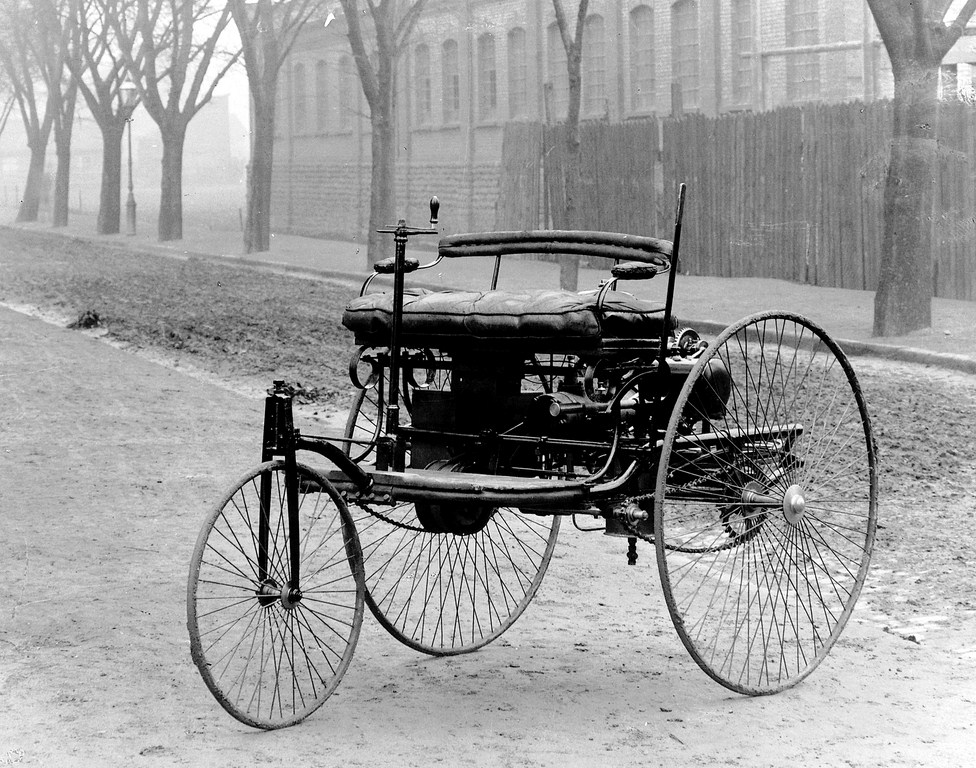
\includegraphics[width=\textwidth]{images/1885Benz.jpg}
    \caption{Benz Patent-Motorwagen (public domain)}
    \label{figure:benz}
\end{figure}
% https://upload.wikimedia.org/wikipedia/commons/7/71/1885Benz.jpg

\begin{figure}[h] \centering
    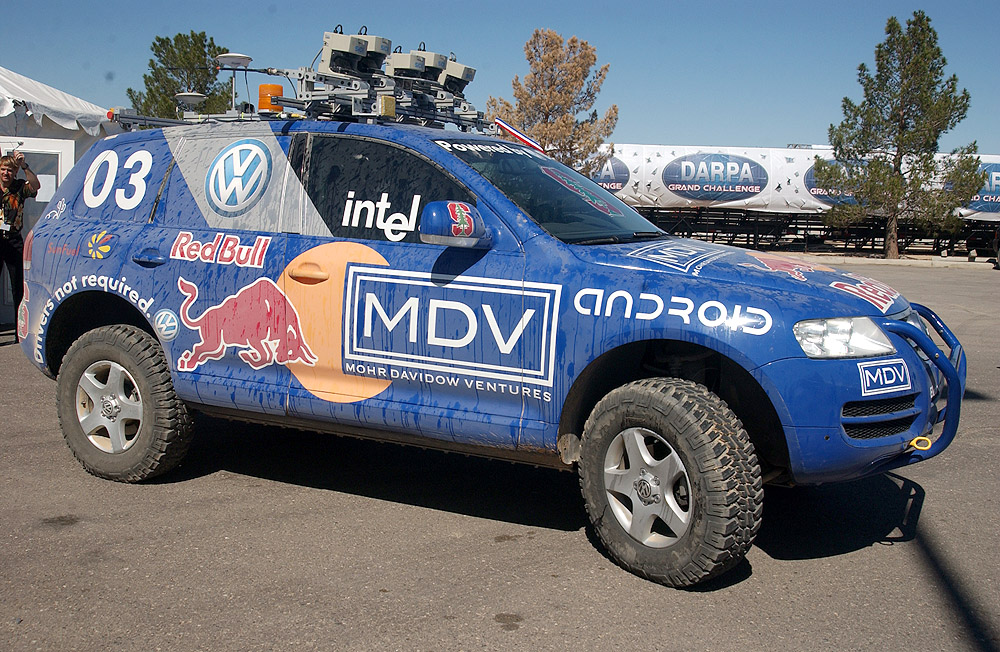
\includegraphics[width=\textwidth]{images/DSC_5090.jpg}
    \caption{Stanley (public domain)}
    \label{figure:stanley}
\end{figure}
% http://archive.darpa.mil/grandchallenge05/grandchallengephotos/awardphotos/DSC_5090.jpg

These two races started a revolution in autonomous vehicles that are completely controlled by computers, not drivers. This drive towards autonomous vehicles, along with complementary technologies like connected, electric, and shared vehicles, has the potential to transform how people travel. Researchers predict these vehicles will increase transportation safety, convenience, access, and efficiency \citep{littman_autonomous_2018, kockelman_implications_2016}. However, these vehicles also present new security risks not found in human-controlled (level 0) vehicles (Table \ref{table:sae_international_taxonomy_2018}). (It is possible for a level 0 car to be equipped with drive-by-wire controls and therefore vulnerable to security risks, but such a configuration is unlikely because it would increase the cost of a vehicle and provide few benefits over mechanical controls.) Consequently, as the number of autonomous vehicles operating on public roads increases, so does the impact of new security risks. This thesis focuses on level 4 and level 5 vehicles because these vehicles do not  expect the driver to respond in any situations. This thesis builds on prior security work inside and outside the automotive industry and presents a security risk assessment framework for autonomous vehicles.

\begin{table}[h]
    \begin{center}
        \begin{tabular}{r l l}
        Level & Name & Dynamic driving task fallback  \\
        \hline
        0 & No Driving Automation & Driver \\
        1 & Driver Assistance & Driver \\
        2 & Partial Driving Automation & Driver \\
        3 & Conditional Driving Automation & Driver \\
        4 & High Driving Automation & System \\
        5 & Full Driving Automation & System
        \end{tabular}
    \caption{Summary of levels of driving automation \citep{sae_international_taxonomy_2018}}
    \label{table:sae_international_taxonomy_2018}
    \end{center}
\end{table}

\subsection{Autonomous and Teleoperated Vehicles}

\begin{mdframed}
    \emph{Programs must be written for people to read, and only incidentally for machines to execute.} \\ -- Harold Abelson \citep{abelson_structure_1996}
\end{mdframed}

\noindent Autonomous vehicles are robotic systems based on the sense, plan, act paradigm (Figure \ref{figure:brooks_robust_1986}) \citep{dickmanns_seeing_1994, christensen_key_2015}. Sensors on the vehicle gather information from the environment. These include lidar, radar, cameras, microphones, and ultrasonic sensors (for slow speeds) \citep{waymo_waymo_2017}. The vehicle's computer systems then combine the sensor inputs to build an understanding about the environment. Next, the vehicle plans its possible actions and compares those possibilities with an overall goal. Planning occurs at several levels: high-level planing including route selection, mid-level planning including lane selection, and low-level planning including vehicle speed and steering angle. The vehicle chooses the best set of actions and actuates electro-mechanical devices to control the vehicle. The entire process continually repeats until the vehicle arrives at its destination.

\begin{figure}[h] \centering
\begin{tikzpicture}[
squarednode/.style={rectangle, draw=black, minimum width=30mm, minimum height=15mm},
]
%Nodes
\node[squarednode](Sense){Sense};
\node[squarednode](Plan)[right=of Sense]{Plan};
\node[squarednode](Act)[right=of Plan]{Act};
\node[squarednode](Environment)[above=of Plan]{Environment};

%Lines
\draw[->] (Sense.east) -- (Plan.west);
\draw[->] (Plan.east) -- (Act.west);
\draw[->] (Act.north) -- (Environment);
\draw[->] (Environment) -- (Sense);
\end{tikzpicture}
    \caption{Sense, plan, act \citep{brooks_robust_1986}}
\label{figure:brooks_robust_1986}
\end{figure}

Teleoperated autonomous vehicles can be controlled by a remote operator that complements or supplements the plan step in an autonomous system. (Teleoperated nonautonomous vehicles also exist but are rare.) In addition to the vehicle, teleoperation requires a command station to control the vehicle from and a communication network for passing information (sense inputs and act outputs) between the vehicle and the command station (Figure \ref{figure:teleoperation}) \citep{tiwari_vehicle_2018}. Teleoperation systems can vary from a simple systems for a robotic taxi booking system that simply informs the vehicle of its destination to a complex system where a remote driver views video from the vehicle's cameras and controls acceleration, braking, and steering of the vehicle \citep{nissan_motor_corporation_press_2017, levinson_teleoperation_2016, okumura_remote_2016, fairfield_remote_2016, rust_expert_2017}. California regulations currently require driverless vehicles to maintain a "communication link between the vehicle and remote operator" \citep{department_of_motor_vehicles_driverless_2018}. To realize cost savings of autonomous vehicles companies would like to operate a greater number of autonomous vehicles than remote operators. The communication link tends to be multiple bonded cellular connections \citep{korosec_82_nodate, korosec_98_nodate}.

\begin{figure}[h] \centering
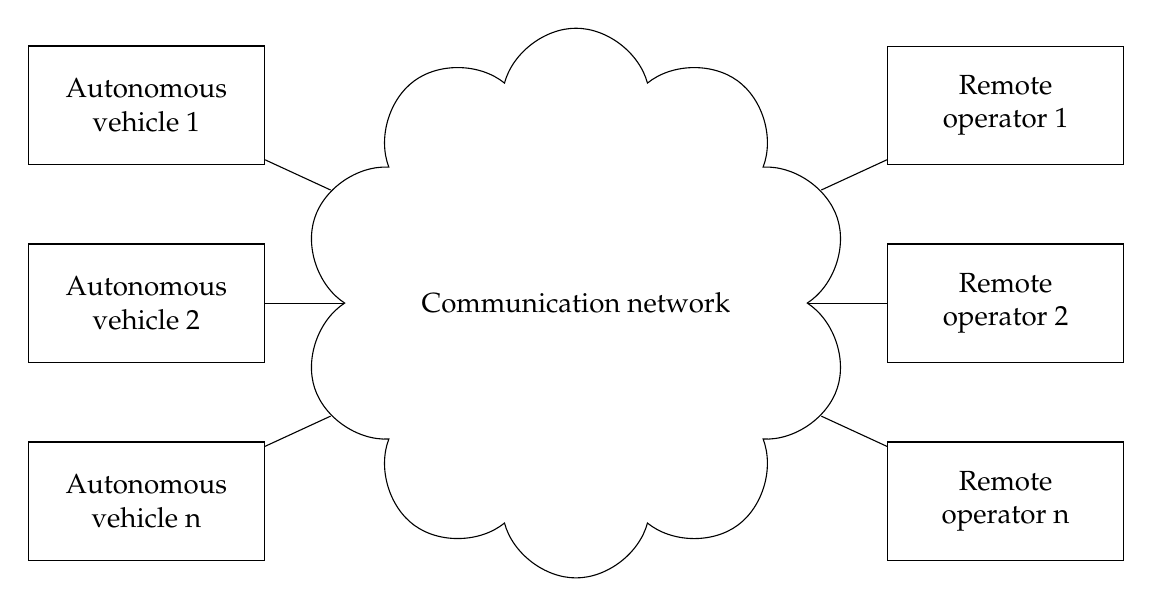
\begin{tikzpicture}[
squarednode/.style={rectangle, draw=black, align=center, minimum width=30mm, minimum height=15mm},
]
%Nodes
\node[squarednode](Autonomous vehicle 1){Autonomous \\ vehicle 1};
\node[squarednode](Autonomous vehicle 2)[below=of Autonomous vehicle 1]{Autonomous \\ vehicle 2};
\node[squarednode](Autonomous vehicle n)[below=of Autonomous vehicle 2]{Autonomous \\ vehicle n};

\node[cloud, draw](Communication network)[right=of Autonomous vehicle 2]{Communication network};

\node[squarednode](Remote operator 2)[right=of Communication network]{Remote \\ operator 2};
\node[squarednode](Remote operator 1)[above=of Remote operator 2]{Remote \\ operator 1};
\node[squarednode](Remote operator n)[below=of Remote operator 2]{Remote \\ operator n};

%Lines
\draw[-] (Autonomous vehicle 1) -- (Communication network);
\draw[-] (Autonomous vehicle 2) -- (Communication network);
\draw[-] (Autonomous vehicle n) -- (Communication network);

\draw[-] (Communication network) -- (Remote operator 1);
\draw[-] (Communication network) -- (Remote operator 2);
\draw[-] (Communication network) -- (Remote operator n);
\end{tikzpicture}
    \caption{Autonomous vehicles and remote operators}
\label{figure:teleoperation}
\end{figure}

\subsection{Information Security and Vehicle Security}

\begin{mdframed}
    \emph{I would give all my fame for a pot of ale, and safety.} -- Boy in Henry V \citep{shakespeare_henry_1599}
\end{mdframed}

% Internet invented by DARPA in 1969 \citep{department_of_defense_department_2015}.

\noindent Historically, computer systems processed information and did not interact with the physical world. Information security risks are classified as threats to \gls{confidentiality} (unauthorized access), \gls{integrity} (unauthorized modifications), and \gls{availability} (uptime) of information (Figure~\ref{figure:cia}) \citep{mccumber_assessing_2004, gordon_official_2015-1}. While confidentiality is often the focus of traditional information security (protecting information from theft), integrity (protecting sensor input data and actuator output commands from tampering) is predicted to be the critical component for systems like autonomous vehicles \citep{schneier_internet_2016}. 

\begin{figure}[h] \centering
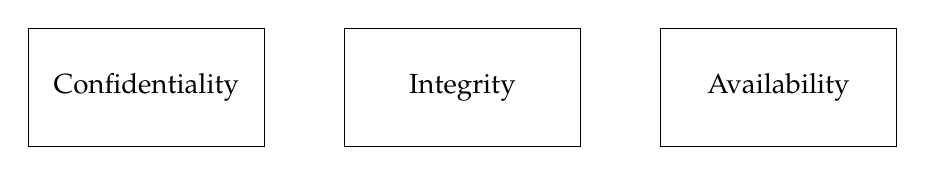
\begin{tikzpicture}[
squarednode/.style={rectangle, draw=black, minimum width=30mm, minimum height=15mm},
]
%Nodes
\node[squarednode](Confidentiality){Confidentiality};
\node[squarednode](Integrity)[right=of Confidentiality]{Integrity};
\node[squarednode](Availability)[right=of Integrity]{Availability};
\end{tikzpicture}
    \caption{The three pillars of information security: \gls{confidentiality, integrity, and availability}}
    \label{figure:cia}
\end{figure}

In the 1980s, the US Department of Defense created policies and standards for securing computer systems \citep{department_of_defense_csc-std-001-83_1983}. Open standards followed years later \citep{holbrook_rfc_1991}, and as computer systems became prevalent in different industries, laws and standards protecting the information processed by these systems quickly followed (Table~\ref{table:laws_standards}). However, only the North American Electric Reliability Corporation's (NERC) Critical Infrastructure Protection (CIP) standards which regulate the electric grid mention control systems that interact with the physical world.

\begin{landscape}
\begin{longtable}{p{10cm} | p{4cm} | p{1.6cm} | p{6cm}}
    Law or Standard & Applicability & Type & Author (Year)\\
    \hline
    California Senate Bill 1386 & California residents & Law & \cite{peace_california_2002} \\
    CIS Controls & Any & Standard & \cite{center_for_internet_security_cis_2018} \\
    Critical Infrastructure Protection standards & North American energy sector & Standard & \cite{north_american_electric_reliability_corporation_critical_} \\
    Family Education Rights and Privacy Act of 1974 (FERPA) & US education sector & Law & \cite{buckley_family_1974} \\
    Federal Information Security Management Act of 2002 (FISMA) & US federal government and contractors & Law & \cite{davis_iii_federal_2002} \\
    General Data Protection Regulation (GDPR) & Individuals located inside the EU & Law & \cite{european_parliament_and_council_regulation_2016} \\
    Gramm-Leach-Bliley Act (GLBA) & US finance sector & Law & \cite{gramm_grammleachbliley_1999} \\
    Health Information Technology for Economic and Clinical Health (HITECH) Act & US healthcare sector & Law & \cite{mcmorris_rodgers_health_2009} \\
    Health Insurance Portability and Accountability Act of 1996 (HIPAA) Security Rule & US healthcare sector & Law & \cite{archer_jr._health_1996}\\
    HITRUST CSF & US healthcare sector & Standard & \cite{hitrust_alliance_hitrust_2018} \\
    International Standard for Assurance Engagements (ISAE) 3402 Assurance Reports on Controls at a Service Organization & Service organizations & Standard & \cite{international_federation_of_accountants_international_2011} \\
    IT Examination Handbook & US finance sector & Standard & \cite{federal_financial_institutions_examination_council_ffiec_it_} \\
    ISO/IEC 27000 family - Information security management systems & International & Standard & \cite{international_organization_for_standardization_iso/iec_2013} \\
    NIST Special Publication 800-53 & US & Standard & \cite{national_institute_of_standards_and_technology_nist_2013} \\
    Payment Card Industry (PCI) Data Security Standards (DSS) & Credit and debit cards & Standard & \cite{pci_security_standards_council_payment_2016} \\
    Sarbanes-Oxley Act of 2002 (SOX) & US public companies & Law & \cite{oxley_sarbanesoxley_2002} \\
    \caption{A sample of information security laws and standards}
    \label{table:laws_standards}
\end{longtable}
\end{landscape}

Information security attacks most often target finance and retail organizations. One simple explanation for this is the quote often misattributed to the bank robber Willie Sutton: "because that's where the money is" \citep{sutton_where_2004}. The transportation industry currently makes up less than 5\% of security breaches \citep{verizon_2017_2017, trustwave_2017_2017}. Nevertheless, the current generation of vehicles controlled by computer systems may contain vulnerabilities, and if malicious individuals exploit these vulnerabilities, they could compromise the computer systems that control a vehicle \citep{koscher_experimental_2010}.

In 2010, researchers from the University of Washington and the University of California, San Diego demonstrated such an attack by controlling the engine, braking, and other systems of a 2009 passenger car \citep{koscher_experimental_2010}.  In 2015 Charlie Miller and Chris Valasek demonstrated a similar attack by remotely controlling the acceleration, braking, steering, and other systems of an unaltered 2014 Jeep Cherokee \citep{miller_remote_2015}. Their research lead to the recall of 1.4 million vehicles and changes to the Sprint wireless carrier network that connected these vehicles to the internet. In 2016, they demonstrated additional attacks that controlled braking and steering systems \citep{miller_advanced_2016}. In 2016, and again in 2017, Keen Security Lab demonstrated another attack where they remotely controlled the infotainment system, windshield wipers, seat controls, mirror controls, door/trunk controls, and braking system of an unaltered Tesla Model S \citep{keen_security_lab_of_tencent_car_2016, keen_security_lab_of_tencent_new_2017}.

Other researchers have also demonstrated attacks against autonomous vehicle sensors and including Global Positioning System receivers \citep{lin_gps_2015}, Lidar \citep{10.1007/978-3-319-66787-4_22}, and several sensors on the Tesla Model S \citep{yan_can_2016}. Additionally, researchers have successfully attacked deep learning models commonly used by autonomous vehicles \citep{evtimov_robust_2017, goodfellow_attacking_2017}. However, no non-research vehicle security attacks have been publicly disclosed. The lack of attacks indicates the advanced skills required for these attacks. However, as the prevalence of autonomous vehicles grows, the motivation to conduct attacks will increase, and therefore the likelihood of attacks will increase.

% This paper uses the term vehicle security instead of the terms automotive security or cybersecurity. Automobiles implies cars with internal combustion engines, but vehicles includes trucks and electric vehicles. Also, cybersecurity typically refers to network security or data security which excludes many of the risks present in vehicles. 

While there are similarities between safety and security (and both words even translate to Sicherheit in German and seguridad in Spanish), this thesis refers to safety as freedom from harm and security as freedom from harm due to actions by external forces. Therefore safety is a broader concept that includes security, but security does not necessarily include accidental harm. Safety systems should include logic and bounds checks \citep{brooks_robust_1986}. For example, a camera that is blinded by a laser can be detected because pixel values would not match those of a road. Additionally, safety systems should prevent vehicles from driving into pedestrians, cyclists, other vehicles, and fixed objects. Last, if the system commands and immediate turn while traveling at highway speeds, the system should reject this command. If these checks fail, the system should default to a safe state such as stopping the vehicle.

\subsection{Risk} \label{subsection:risk}
\begin{mdframed}
    \emph{The best-laid schemes o' mice an' men / Gang aft agley. \\ (The best-laid plans of mice and men / Go oft awry.)} -- Robert \cite{burns_mouse_1785}
\end{mdframed}

\noindent Federal Information Processing Standard 200 defines risk as "a measure of the extent to which an entity is threatened by a potential circumstance or event, and typically a function of: (i) the adverse impacts that would arise if the circumstance or event occurs; and (ii) the likelihood of occurrence" \citep{national_institute_of_standards_and_technology_federal_2006}. Similarly, ISO 31000 defines risk as "effect of uncertainty on objectives," which implies that risk is neither positive or negative \citep{international_organization_for_standardization_iso_2018}. Risk is defined in Equation~\ref{equation:risk}.

\begin{equation}
    Risk = Impact \times Likelihood
    \label{equation:risk}
\end{equation}

NIST Special Publication 800-30 describes risk as a \gls{threat source} which initiates a \gls{threat event} which exploits a \gls{vulnerability} which causes an \gls{adverse impact} which produces \gls{organizational risk} (Figure \ref{figure:generic_risk_model}) \citep{national_institute_of_standards_and_technology_nist_2012}. The publication defines four categories for threat sources (adversarial, accidental, structural, and environmental) \citep[Appendix D]{national_institute_of_standards_and_technology_nist_2012} and two categories for threat events (adversarial and non-adversarial) \citep[Appendix E]{national_institute_of_standards_and_technology_nist_2012}.  This process again demonstrates how risk is a combination of an impact and a likelihood of a threat source initiating a threat event which exploits a vulnerability. Adverse impact is typically a loss of confidentiality, integrity, or availability of information.

\begin{figure}[h] \centering
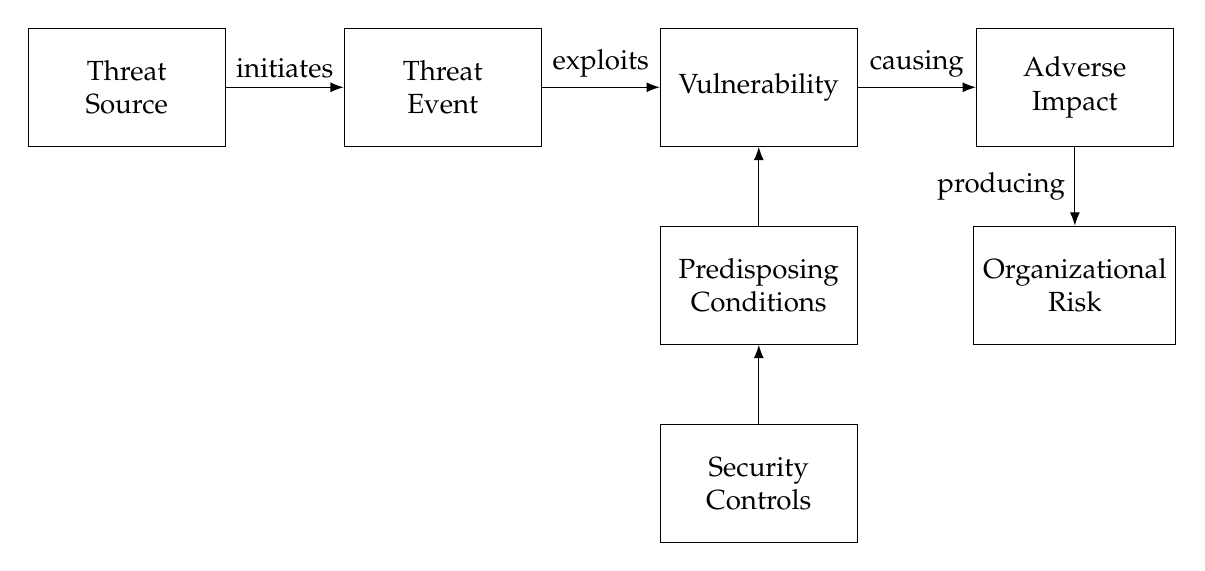
\begin{tikzpicture}[
squarednode/.style={rectangle, align=center, draw=black, minimum width=25mm, minimum height=15mm},
]
%Nodes
\node[squarednode](Threat Source){Threat \\ Source};
\node[squarednode](Threat Event)[right=1.5cm of Threat Source]{Threat \\ Event};
\node[squarednode](Vulnerability)[right=1.5cm of Threat Event]{Vulnerability};
\node[squarednode](Predisposing Conditions)[below= of Vulnerability]{Predisposing \\ Conditions};
\node[squarednode](Security Controls)[below= of Predisposing Conditions]{Security \\ Controls};
\node[squarednode](Adverse Impact)[right=1.5cm of Vulnerability]{Adverse \\ Impact};
\node[squarednode](Organizational Risk)[below=of Adverse Impact]{Organizational \\ Risk};

%Lines
\draw[->] (Threat Source) -- node [above] {initiates} (Threat Event);
\draw[->] (Threat Event) -- node [above] {exploits} (Vulnerability);
\draw[->] (Vulnerability) -- node [above] {causing} (Adverse Impact);
\draw[->] (Predisposing Conditions) -- (Vulnerability);
\draw[->] (Security Controls) -- (Predisposing Conditions);
\draw[->] (Adverse Impact) -- node [left] {producing} (Organizational Risk);
\end{tikzpicture}
    \caption{Generic risk model \citep{national_institute_of_standards_and_technology_nist_2012}}
\label{figure:generic_risk_model}
\end{figure}

\subsection{Controls} \label{subsection:controls}

\begin{mdframed}
    \emph{The ultimate cause of our failure was a simple one: despite all statements to the contrary, it was not due to lack of bravery on the part of our men, or to any fault of the Fleet's. We were defeated by one thing only -- by the inferior science of our enemies. I repeat -- by the inferior science of our enemies.} -- Arthur C. \cite{clarke_superiority_1951}
\end{mdframed}

NIST Special Publication 800-53 defines security controls as "the safeguards/countermeasures prescribed for information systems or organizations that are designed to: (i) protect the confidentiality, integrity, and availability of information that is processed, stored, and transmitted by those systems/organizations; and (ii) satisfy a set of defined security requirements" \citep{national_institute_of_standards_and_technology_nist_2013}. Controls can be classified as administrative, technical, or physical. Table \ref{enumerate:national_institute_of_standards_and_technology_nist_2013} lists the Security Control Identifiers from NIST Special Publication 800-53. Charlie McCarthy and Kevin Harentt believe the vehicle sector should develop a "Security Control Catalog" based on NIST Special Publication 800-53 similar to the guides available for energy, control systems, and public transportation industries \citep{mccarthy_national_2014}. In GM's comments on NHTSA's Guidelines for the Safe Deployment and Operation of Automated Vehicle Safety Technologies, they propose a controls including "security design reviews and penetration testing, designing and understanding system defensive measures, and the development of monitoring, detection, and response capabilities" \citep{national_highway_traffic_safety_administration_guidelines_2016}. Other common lists of controls are the CIS Controls from the Center for Internet Security (Figure \ref{enumerate:center_for_internet_security_cis_2018}) and the PCI Data Security Standard -- High Level Overview from the Payment Card Industry (Table \ref{table:pci_security_standards_council_payment_2016}). Adding controls modifies the risk equation (Equation \ref{equation:risk}) by adding a controls factor (Equation \ref{equation:residual_risk}). 
 
 \begin{equation}
    Residual\ Risk = Impact \times Likelihood \times Controls
    \label{equation:residual_risk}
\end{equation}

\subsection{Risk Management}

\begin{mdframed}
    \emph{Risk Management: It's not rocket science - it's much more complicated.} -- John \cite{adams_risk_2005}
\end{mdframed}

\noindent \gls{Risk Management} is an organizational process to measure and manage risk. NIST Special Publication 800-37 defines the \gls{Risk Management Framework} (Figure \ref{figure:national_institute_of_standards_and_technology_nist_2017}) which is a common risk management framework. ISO/IEC 27005 - Information security risk management provides an alternative to NIST's framework, but is not freely available \citep{international_organization_for_standardization_iso/iec_2018}. The Federal Information Security Management Act of 2002 (FISMA) requires federal organizations to follow the Risk Management Framework to manage information security risks \citep{davis_iii_federal_2002}. McCarthy and Harnett modified the Risk Management Framework into the Risk Management Framework for the Vehicle Sector (Figure \ref{figure:mccarthy_national_2014}) \citep{mccarthy_national_2014}. In Google's comments on NHTSA's Guidelines for the Safe Deployment and Operation of Automated Vehicle Safety Technologies, they propose a risk management approach: "self driving vehicles should be designed with a process that can identify known threats (malicious or otherwise) to the vehicle's electronic systems and explain how they have been mitigated by design (e.g. Google's web services use ISO 27001:2013 to validate the design of their security risk management processes)" \citep{national_highway_traffic_safety_administration_guidelines_2016}. \\

\begin{figure}[h] \centering
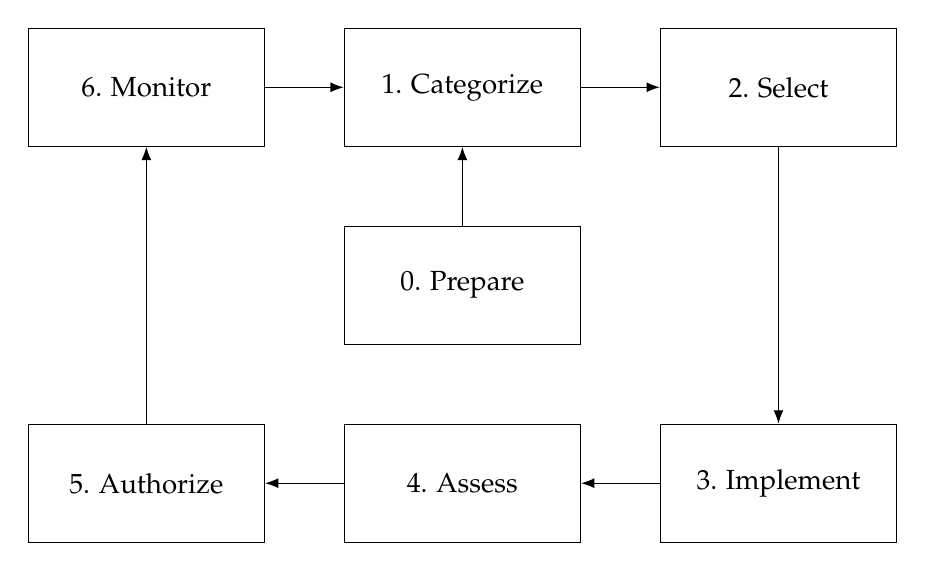
\begin{tikzpicture}[
squarednode/.style={rectangle, align=center, draw=black, minimum width=30mm, minimum height=15mm},
]
%Nodes
\node[squarednode](Prepare){0. Prepare};
\node[squarednode](Categorize)[above= of Prepare]{1. Categorize};
\node[squarednode](Select)[above right= of Prepare]{2. Select};
\node[squarednode](Implement)[below right= of Prepare]{3. Implement};
\node[squarednode](Assess)[below= of Prepare]{4. Assess};
\node[squarednode](Authorize)[below left= of Prepare]{5. Authorize};
\node[squarednode](Monitor)[above left= of Prepare]{6. Monitor};

%Lines
\draw[->] (Prepare) -- (Categorize);
\draw[->] (Categorize) -- (Select);
\draw[->] (Select) -- (Implement);
\draw[->] (Implement) -- (Assess);
\draw[->] (Assess) -- (Authorize);
\draw[->] (Authorize) -- (Monitor);
\draw[->] (Monitor) -- (Categorize);
\end{tikzpicture}
    \caption{Risk Management Framework \citep[Page 8]{national_institute_of_standards_and_technology_nist_2017}}
\label{figure:national_institute_of_standards_and_technology_nist_2017}
\end{figure}

\begin{figure}[h] \centering
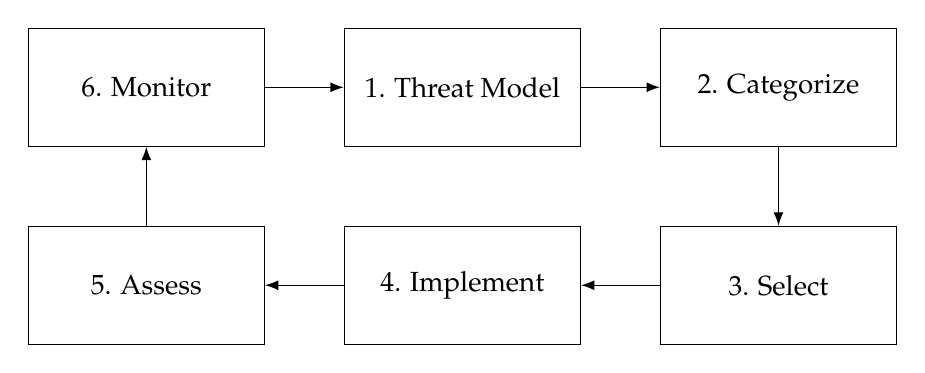
\begin{tikzpicture}[
squarednode/.style={rectangle, align=center, draw=black, minimum width=30mm, minimum height=15mm},
]
%Nodes
\node[squarednode](Threat Model){1. Threat Model};
\node[squarednode](Categorize)[right= of Threat Model]{2. Categorize};
\node[squarednode](Select)[below= of Categorize]{3. Select};
\node[squarednode](Implement)[below= of Threat Model]{4. Implement};
\node[squarednode](Assess)[left= of Implement]{5. Assess};
\node[squarednode](Monitor)[left= of Threat Model]{6. Monitor};

%Lines
\draw[->] (Threat Model) -- (Categorize);
\draw[->] (Categorize) -- (Select);
\draw[->] (Select) -- (Implement);
\draw[->] (Implement) -- (Assess);
\draw[->] (Assess) -- (Monitor);
\draw[->] (Monitor) -- (Threat Model);
\end{tikzpicture}
    \caption{Risk Management Framework for the Vehicle Sector \citep{mccarthy_national_2014}}
\label{figure:mccarthy_national_2014}
\end{figure}

Risk management is common in many industries as a way to protect an organization from uncertainty. Risks could be financial risk, strategic risk, political risk, or other types of risk. This thesis chooses to focus on security risk because of the unique applicability to autonomous vehicle systems and excludes other types of risk. Organizations have four options for handling risks once identified:
\begin{itemize}
    \item Avoidance: eliminate the cause of the risk
    \item Control: implement controls to reduce the risk
    \item Transferance: contract with a third party to buy insurance against the risk, hedge against the risk, or outsource the risk
    \item Acceptance: accept the risk
\end{itemize}
Scope is an important tool in risk management. Limiting the size of a system or the number of interconnected systems can greatly reduce the impact of risk and therefore the overall risk management process. This is addressed during the categorization step of the risk management framework along with security level classification of the system. For example, a mobile application is public and accessible to everyone, but vehicle's internal control systems need additional controls to protect them. Classifications are common for computer information systems \citep{markiewicz_guidelines_2015, stanford_university_it_risk_}.

Another import concept in risk management is \gls{defense in depth} where multiple redundant layers of security controls provide redundancy in case one or more security controls fails \citep{gordon_official_2015-1}. Defense in depth is also called the onion model where layers of an onion represent layers of security controls. The Swiss cheese model elaborates on this concept by describing each layer of security as a piece of cheese where the holes are vulnerabilities. A system failure requires the holes from all layers of cheese to align.

\subsection{Risk Assessment} \label{section:risk_assessment}

\begin{mdframed}
\emph{The revolutionary idea that defines the boundary between modern times and the past is the mastery of risk: the notion that the future is more than a whim of the gods and that men and women are not passive before nature. Until human beings discovered a way across that boundary, the future was the mirror of the past or the murky domain of oracles and soothsayers who held a monopoly over knowledge of anticipated events.} -- Peter \cite{bernstein_against_1998}
\end{mdframed}

\noindent A risk assessment is a tool for measuring risk in a system. NIST Special Publication 800-30 defines the end result of a risk assessment as "a determination of risk (i.e., typically a function of the degree of harm and likelihood of harm occurring)" \citep[page 1]{national_institute_of_standards_and_technology_nist_2012}. NIST Special Publication 800-30 publication defines a process for a risk assessment (Figure \ref{figure:national_institute_of_standards_and_technology_nist_2012}). This process is used as the basis of section \ref{section:methods}.

\begin{figure}[h]
    \begin{enumerate}
        \item Prepare for Assessment
        \item Conduct Assessment
        \begin{enumerate}
            \item Identify threat sources and events
            \item Identify vulnerabilities and predisposing conditions
            \item Determine likelihood of occurrence
            \item Determine magnitude of impact
            \item Determine risk
        \end{enumerate}
        \item Communicate Results
        \item Maintain Assessment 
    \end{enumerate}
    \caption{Risk Assessment Process \citep{national_institute_of_standards_and_technology_nist_2012}}
\label{figure:national_institute_of_standards_and_technology_nist_2012}
\end{figure}

\newpage
\subsection{Risk Quantification}

\begin{mdframed}
    \emph{I often say that when you can measure what you are speaking about, and express it in numbers, you know something about it; but when you cannot measure it, when you cannot express it in numbers, your knowledge is of a meagre and unsatisfactory kind; it may be the beginning of knowledge, but you have scarcely, in your thoughts, advanced to the stage of science, whatever the matter may be.} -- Lord Kelvin \citep{thomson_1st_baron_kelvin_electrical_1883}
\end{mdframed}

\noindent NIST Special Publication 800-30 provides qualitative table (Table \ref{national_institute_of_standards_and_technology_nist_2012_assessment_scale}) for computing risk from likelihood and impact values. Risk values from "Very Low" to "Very High" map to a qualitative scale and semi-quantitative (ordinal) scales  (Table \ref{national_institute_of_standards_and_technology_nist_2012_level_of_risk}). There are numerous other risk measures including the Common Vulnerability Scoring System (CVSS), Microsoft's DREAD model, the OWASP Risk Rating Methodology, MIL-STD-882E - System Safety, and the Automotive Safety Integrity Level (ASIL) (Table \ref{table:risk_measures}).

\begin{table}[h]\begin{center}
    \begin{tabular}{c | c | c | c | c | c}
Likelihood & \multicolumn{5}{c}{Level of Impact} \\
 & Very Low & Low & Moderate & High & Very High \\
\hline
Very High & Very Low & Low &  Moderate & High &  Very High \\
High & Very Low & Low & Moderate & High & Very High \\
Moderate & Very Low & Low & Moderate & Moderate & High \\
Low & Very Low & Low & Low & Low & Moderate \\
Very Low & Very Low & Very Low & Very Low & Low & Moderate \\
    \end{tabular}
    \caption{Assessment Scale - Level of Risk  \citep[page I-1]{national_institute_of_standards_and_technology_nist_2012}}
    \label{national_institute_of_standards_and_technology_nist_2012_assessment_scale}
\end{center} \end{table}

\begin{table}[p]\begin{center}
    \begin{tabularx}{\linewidth}{c | c | c | X}
        Qualitative Values & \multicolumn{2}{c |}{Semi-Quantitative Values} & Description \\
        \hline
        Very High & \hphantom{aa} 96-100 \hphantom{aa} & 10 & Very high risk means that a threat event could be expected to have multiple severe or catastrophic adverse effects on organizational operations, organizational assets, individuals, other organizations, or the Nation. \\
        High & 80-95 & 8 & High risk means that a threat event could be expected to have a severe or catastrophic adverse effect on organizational operations, organizational assets, individuals, other organizations, or the Nation. \\
        Moderate & 21-79 & 5 & Moderate risk means that a threat event could be expected to have a serious adverse effect on organizational operations, organizational assets, individuals, other organizations, or the Nation. \\
        Low & 5-20 & 2 & Low risk means that a threat event could be expected to have a limited adverse effect on organizational operations, organizational assets, individuals, other organizations, or the Nation. \\
        Very Low & 0-4 & 0 & Very low risk means that a threat event could be expected to have a negligible adverse effect on organizational operations, organizational assets, individuals, other organizations, or the Nation. \\
    \caption{Assessment Scale - Level of Risk  \citep[page I-2]{national_institute_of_standards_and_technology_nist_2012}}
    \label{national_institute_of_standards_and_technology_nist_2012_level_of_risk}
    \end{tabularx}
\end{center} \end{table}

\newpage
\begin{landscape}
\begin{longtable}{p{5cm} | p{4cm} | p{8cm} | p{5cm}}
Framework & Scale & Mesures & Author \\ \hline
NIST Special Publication 800-30 & qualitative and semi-quantitative (ordinal) & likelihood, impact                                                                                                                                                                                                                                                                                                                                                                                                                                                             & \cite{national_institute_of_standards_and_technology_nist_2012} \\
Common Vulnerability Scoring System & semi-quantitative (0-10) & attack vector, attack complexity, privilege required, user interaction, C,I,A impact, exploit code maturity, remediation level, report confidence, and security requirements                                                                                                                                                                                                                                                        & \cite{first.org_inc._common_2015} \\
Microsoft's DREAD & semi-quantitative (1-10) & damage, reproducibility, exploitability, affected users, and discoverability                                                                                                                                                                                                                                                                                                                                                                                   & \cite{leblanc_dreadful_2007} \\
OWASP Risk Rating Methodology & qualitative and semi-quantitative (0-9) & likelihood based on threat agent factors and vulnerability factors,  impact based on technical impact factors and business impact factors & \cite{open_web_application_security_project_owasp_2016} \\
MIL-STD-882E - System Safety & qualitative & severity, probability                                                                                                                                                                                                                                                                                                                                                                                                                                                          & \cite{department_of_defense_mil-std-882e_2012} \\
Automotive Safety Integrity Level (ASIL) & qualitative & probability, severity, and controllability                                                                                                                                                                                                                                                                                                                                                                                                                                     & \cite{international_organization_for_standardization_iso_2011} \\
    \caption{A sample of risk measures}
    \label{table:risk_measures}
\end{longtable}
\end{landscape}

However, these methods are all "handicapped by a reliance on non-quantitative methodologies" \citep{soo_hoo_how_2000}. Qualitative and semi-quantitative risk scales all suffer from problems of interpretability (e.g. Does a highly likely event have a 50\%, 60\%, 70\%, 80\%, or 90\% probability of occurring?) and computation (e.g. Are three medium risk events worse than one high risk event?) \citep[chapter 5]{hubbard_how_2016}. Hubbard and Seiersen recommend quantitative (ratio scale) risk assessments based on the probability (likelihood) and impact (dollars) of threat events. Other companies use a quantitative scale based on the value of bug bounty programs \citep{held_measuring_2017}.

\subsection{Research Questions and Contributions}

This goal of this thesis is to provide insight and answers to several questions regarding the security of autonomous vehicle systems:

\begin{enumerate}
\item Can risk management frameworks quantitatively measure the security risks of autonomous vehicle systems? 
\item Can risk management frameworks help manufacturers of autonomous vehicle systems prioritize security controls for these systems?
\item Can risk management frameworks provide assurances that autonomous vehicle systems are secure against cyberattacks?
\end{enumerate}

This thesis contributes several original risk management techniques and example applications of those techniques. This thesis presents the first risk assessment of an autonomous vehicle system. This is the first time that a threat assessment has been applied to an autonomous vehicle system to determine the likelihood and impacts of security risks. Additionally, it is the first time that risk reduction through controls has been evaluated as part of such a risk assessment.

This thesis is also one of the first applications of quantitative risk management techniques to the security community. While quantitative techniques are popular in finance, security assessments often rely on qualitative methods which have many drawbacks listed above. This thesis uses quantitative methods to overcome those drawbacks and quantify the potential security impacts of autonomous vehicle systems. Additionally, this is the first time optimization methods have been used to select the optimal security controls to reduce risk in an autonomous vehicle system.

Last, this thesis provides a method for manufacturers of autonomous vehicle systems to provide assurances that the security risks in their systems are as low as reasonably practicable. This is an important step in public acceptance of autonomous vehicle systems.

\subsection{Structure of the Thesis}

The methods of this thesis are based on an adaptation of NIST Special Publication 800-30 risk assessment process (Figure \ref{figure:national_institute_of_standards_and_technology_nist_2012}) using quantitative methods instead of qualitative methods. This adapted framework provides the ability to compute risk using either discrete methods based on mean likelihoods and impacts or stochastic methods based on Monte Carlo simulations of likelihood and impact distributions. A controls selection step is added after the assessment which uses simple optimization techniques to balance the costs of controls and the expected loss from the risks they mitigate. 

The results section describes the risk assessment and controls selection process for a sample autonomous vehicle system. The results contain many examples of controls that mitigate one or several risks. These examples provide several scenarios for control selection. Some scenarios reduce the expected loss greater than their cost of their controls and some do not. An expected loss curve is also presented for a base scenario with no controls and a optimal controls scenario. As this is an example system there are numerous assumptions behind the risks and controls.

The discussion focuses on areas where the autonomous vehicles industry can improve its security posture and how risk management fits into the overall security picture. Additionally, areas where this thesis is lacking and areas for future research are discussed.

\newpage
\section{Methods} \label{section:methods}
\noindent This process generally follows the Risk Assessment Process from NIST Special Publication 800-30 (Figure \ref{figure:national_institute_of_standards_and_technology_nist_2012}), but uses quantitative values in place of qualitative scales. A risk assessment library was created in the python programming language for all computations \citep{bailey_rail_2018}. \\

\begin{mdframed}
\emph{The Three Laws of Robotics \\
1. A robot may not injure a human being or, through inaction, allow a human being to come to harm. \\
2. A robot must obey the orders given it by human beings except where such orders would conflict with the First Law. \\
3. A robot must protect its own existence as long as such protection does not conflict with the First or Second Laws. \\}
-- Isaac \cite{asimov_runaround_1950}
\end{mdframed}

\subsection{Prepare for Assessment}

\begin{mdframed}
    \emph{When you fail to prepare, you're preparing to fail.} -- John Wooden \citep{cromwell_wooden_1977}
\end{mdframed}

\noindent The tasks in preparation for the assessment are to identify the purpose (desired outputs), scope, assumptions and constraints, information sources, and risk model and analytic approach for the risk assessment \citep[pages 24-28]{national_institute_of_standards_and_technology_nist_2012}. Similar to how the PCI Data Security Standards define their scope as the "people, processes and technologies that store, process, or transmit cardholder data or sensitive authentication data," a vehicle assessment's scope include any people, processes, and technologies that could be used to control a vehicle \citep{pci_security_standards_council_payment_2016}. Ford considers the scope of their security program to include "not only to the vehicles' electronics, sensors and Virtual Driver System but also to any feature connected to them" \citep[page 35]{ford_motor_company_matter_2018}. Also, Miller and Valasek demonstrated the scope of the Jeep Cherokee they hacked was not limited by proximity to the vehicle when they remotely connected to the vehicle via the internet and were able to control it \citep{miller_remote_2015}. Assessments can be simplified by separating the system into subsystems and with subsystem boundaries and assessing the individual subsystems and the boundaries \citep[page 13]{national_institute_of_standards_and_technology_nist_2017}. This is recommended to reduce scope, cost, difficulty, and risk \citep[page 11]{pci_security_standards_council_payment_2016}.

\subsection{Conduct Assessment}

The generic risk model (Figure \ref{figure:generic_risk_model}) can be represented as figure \ref{figure:risk_model} to match the risk assessment process.

\begin{figure}[h] \centering
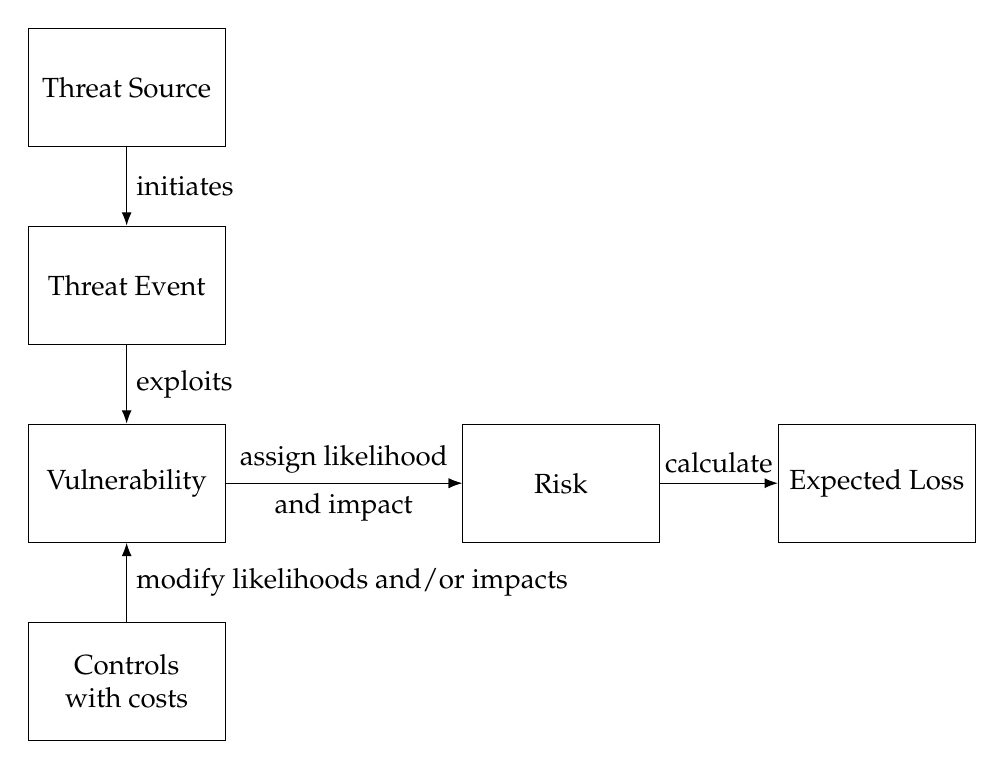
\begin{tikzpicture}[
squarednode/.style={rectangle, align=center, draw=black, minimum width=25mm, minimum height=15mm},
]
%Nodes
\node[squarednode](Vulnerability){Vulnerability};
\node[squarednode](Threat Event)[above=of Vulnerability]{Threat Event};
\node[squarednode](Threat Source)[above=of Threat Event]{Threat Source};
\node[squarednode](Risk)[right=3cm of Vulnerability]{Risk};
\node[squarednode](Controls)[below=of Vulnerability]{Controls\\ with costs};
\node[squarednode](Expected Loss)[right=1.5cm of Risk]{Expected Loss};

%Lines
\draw[->] (Threat Source) -- node [right] {initiates} (Threat Event);
\draw[->] (Threat Event) -- node [right] {exploits} (Vulnerability);
\draw[->] (Vulnerability) -- node [above] {assign likelihood} (Risk);
\draw[->] (Vulnerability) -- node [below] {and impact} (Risk);
\draw[->] (Controls) -- node [right] {modify likelihoods and/or impacts} (Vulnerability);
\draw[->] (Risk) -- node [above] {calculate} (Expected Loss);

\end{tikzpicture}
    \caption{Risk model}
\label{figure:risk_model}
\end{figure}

\subsubsection{Identify threat sources and events}  \label{section:identify_threat_sources_and_events}

Generally, \gls{threat source}s can be grouped into two categories: adversarial and non-adversairal \citep{national_institute_of_standards_and_technology_nist_2012}. Threat events are a function of threat sources (Equation \ref{equation:threat_event}).

\begin{equation}
    Threat\ Event = f(Threat\ Source)
    \label{equation:threat_event}
\end{equation}

NIST Special Publication 800-30 provides threat event categories and sample threat events (Figure \ref{enumerate:national_institute_of_standards_and_technology_nist_2012-E}). Petit and Shladover created threat models for autonomous and connected vehicles. They determined the attack surface for autonomous vehicles to consist of infrastructure signs, machine vision, GPS, in-vehicle devices, acoustic sensors, radar, lidar, roads, in-vehicle sensors, odometric sensors, electronic devices, and maps \citep{petit_potential_2015}. However they do not include any teleoperation capabilities that are now common in autonomous vehicles or assign a likelihood or impact to any attacks.

\begin{figure}[h]
Threat Events
\begin{itemize}
  \item Adversarial threat events
    \begin{itemize}
        \item Perform reconnaissance and gather information.
        \item Craft or create attack tools.
        \item Deliver/insert/install malicious capabilities.
        \item Exploit and compromise.
        \item Conduct an attack (i.e., direct/coordinate attack tools or activities).
        \item Achieve results (i.e., cause adverse impacts, obtain information)
        \item Maintain a presence or set of capabilities.
        \item Coordinate a campaign.
    \end{itemize}
  \item Non-adversarial threat events
    \end{itemize}
\caption{Threat event categories \citep[Appendix E]{national_institute_of_standards_and_technology_nist_2012}}
    \label{enumerate:national_institute_of_standards_and_technology_nist_2012-E}
\end{figure}


Other organizations such as Germany's Federal Office for Information Security (Bundesamt f\"{u}r Sicherheit in der Informationstechnik), the Cloud Security Alliance, and the Open Web Application Security Project (OWASP) have created threat catalogs \citep{bundesamt_fur_sicherheit_in_der_informationstechnik_elementary_2008, cloud_security_alliance_top_threats_working_group_treacherous_2016, open_web_application_security_project_owasp_2017}. Additionally, several books list hacking methodologies that can be helpful for brainstorming additional threats \citep{mcnab_network_2007, smith_car_2016}.

Threats to autonomous vehicles can also be classified according to if they attack the sense, plan, or act systems, or the environment (Figure \ref{figure:brooks_robust_1986}). Traditional information security models such as the OSI model or the Internet model (Table \ref{table:osimodel_internetmodel}) are helpful for grouping different threats. Last, data flow diagrams can help trace information through an information system. Similarly, for control systems such as autonomous vehicles, control flow diagrams describe the flow of information within these systems.

\begin{table}[h]\begin{center}
    \begin{tabular}{l | l}
        OSI model & Internet model \\
        \hline
        7. Application & Application \\
        6. Presentation & \\
        5. Session & \\
        4. Transport & Transport \\
        3. Network &  Internet \\
        2. Data link &  \\
        1. Physical & Link \\
    \end{tabular}
    \caption{OSI model \citep{international_organization_for_standardization_iso/iec_1994} and Internet model \citep{braden_rfc_1989}}
    \label{table:osimodel_internetmodel}
\end{center} \end{table}

All of the above inputs were combined to form a threat model (Table \ref{table:results}) for an example autonomous vehicle system (Figure \ref{autonomous_vehicle_system}). Threat sources are a class in the risk assessment library. Threat events are a class which depend on a threat source.

\subsubsection{Identify vulnerabilities and predisposing conditions}
Vulnerabilities are a function of threat events, security controls, and a system (with predisposing conditions) (Equation \ref{equation:vulnerability}). Controls each come with a cost and can modify either the impact or likelihood of a risk. Additionally, controls often do not reduce risk to zero, but rather by some factor. For example, anti-malware software will prevent infection from some malware, but not zero-day attacks \citep{vegge_where_2009}. Also, passwords, another common control, are vulnerable to guessing, observing, viewing when written down, and more \citep{bryant_user_2006}. Eliminating a vulnerability can reduce the risk of that vulnerability to zero.

The concept of a kill chain can help in identifying vulnerabilities. The phases of a kill chain (reconnaissance, weaponization, delivery, exploitation, installation, command and control, action on objectives) show how attacks must be successful in all phases to create risk while defenses may block an attack at any phase \citep[page 19]{pols_unified_2017}. McNab offers three simpler phases (reconnaissance, enumeration, and exploration) to an attack \citep{mcnab_network_2007}.

\begin{equation}
    Vulnerability = f(Threat\ Event,\ Controls,\ System)
    \label{equation:vulnerability}
\end{equation}

As described in equation \ref{equation:vulnerability}, the threat model from section \ref{section:identify_threat_sources_and_events} generates vulnerabilities. In the risk assessment library, vulnerabilities are a class which depend on a threat event, system, and controls. Systems are a tree which describe the autonomous vehicle system. Controls are a class which have a cost and a reduction factor. They also have a boolean to determine if they are implemented or not for use in calculations and optimizations.

\subsubsection{Determine likelihood of occurrence}

Likelihoods are defined as the number of expected occurrences per year. We represent likelihoods by a Poisson distribution because they are discrete and positive. Likelihoods are a function of vulnerabilities which themselves are a function of threat events, controls, and systems (Equation \ref{equation:likelihood}). Likelihoods can be determined by analysis of historical data or expert surveys \citep{joh_defining_2017}. Two example likelihood histograms are show in Figure \ref{figure:likelihoods} representing .5 events/year and 100 events/year.

\begin{equation}
    Likelihood = f(Vulnerability)
    \label{equation:likelihood}
\end{equation}

In the risk assessment library, likelihoods are a class defined by the lambda of the Poisson distribution.

\begin{figure}[h] \centering
    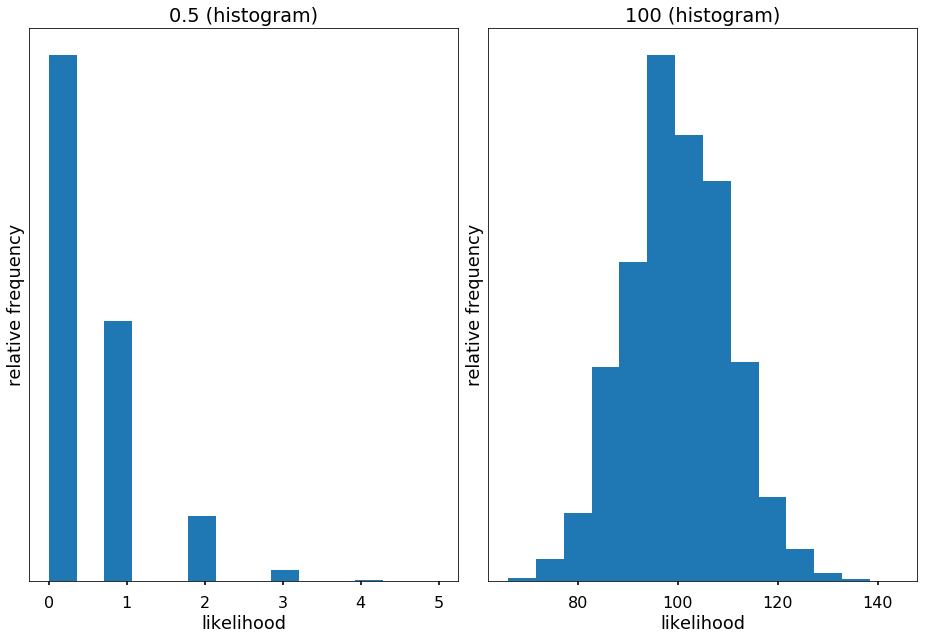
\includegraphics[width=\textwidth]{images/likelihoods.png}
    \caption{Example likelihood distributions}
    \label{figure:likelihoods}
\end{figure}

\subsubsection{Determine magnitude of impact}

Impacts are losses defined by monetary units such as United States dollars or euros. These losses are represented by log normal distributions because they are continuous, positive, and have a long tail \citep{hubbard_how_2016}. Impacts, like likelihoods, are a function of vulnerabilities (Equation \ref{equation:impact}). Impacts can be determined by analysis of historical data or expert surveys \citep{joh_defining_2017}.

Quantitative risk modeling is common in the financial sector and there is quite a large amount of research on financial impacts. One main difference between finance and security is the type of impacts. Financial models define risk as both profit and loss: an investment has the potential to increase or decrease in value \citep{embrechts_lectures_2005, mcneil_quantitative_2015}. However, for  security risk, we are only concerned with losses. The same is true for transportation safety models such as a road safety models where impacts may be defined in fatalities or crashes.

\begin{equation}
    Impact = f(Vulnerability)
    \label{equation:impact}
\end{equation}

Impacts to autonomous vehicles can be classified into a few broad categories: attacks where an attacker compromises the control systems of a vehicle to cause an intentional crash, attacks where an attacker causes these systems to fail uncontrollably and the vehicle to crash, and attacks which disable these systems and the vehicle. Additionally, these attacks may involve one vehicle or an entire fleet of vehicles.  Other attacks may have impacts similar to traditional information security attacks such as information theft.

In the risk assessment library, impacts are a class defined by the mu and sigma terms of the log normal distribution. There is and additional method for defining an impact based on the lower 90\% and upper 90\% confidence interval.

\subsubsection{Determine risk} \label{subsubsection:determine_risk}

Risk is calculated by both deterministic and stochastic methods. Deterministic values are calculated from the mean likelihood and mean impact of each risk using the residual risk equation (Equation \ref{equation:residual_risk}) from section \ref{subsection:controls}. Stochastic risk values are calculated from random sampling of likelihood and impact distributions, again using the residual risk equation. Using the stochastic risk values, a Monte Carlo simulation, over thousands of iterations, samples values of the residual risk at each iteration \citep[page 477]{carey_risks_2006}. The result of a deterministic calculation is one value, the annualized expected loss mean, and the result of a stochastic calculation is a probability density function of annualized expected loss. The annualized expected loss is the summation of all residual risks to the autonomous vehicle system (Equation \ref{equation:annual_expected_loss}).

\begin{equation}
    Annual\ Expected\ Loss = \sum Residual\ Risk
    \label{equation:annual_expected_loss}
\end{equation}

In the risk assessment library, risks are a class defined by a vulnerability, likelihood, and impact. There are methods to calculate deterministic and stochastic risk values as defined above. There are also methods to perform Monte Carlo simulations of stochastic risk values. For all methods, controls may be implemented or not.
\subsection{Communicate Results}

The result of the risk assessment, as mentioned in section \ref{section:risk_assessment}, is a determination of risk. In a deterministic calculation, this is the annualized expected loss of the system. The Monte Carlo simulation results in a distribution of annualized expected loss. Additional controls can be evaluated based upon their cost effectiveness. Additionally, these results can be compared with an organization's risk tolerance to determine if additional controls, perhaps cost ineffective, should be implemented.

In the risk assessment library, a risks class is defined by all the risks of a system. This class has a method to calculate the mean annualized expected loss of a system and a method to calculate and plot the annualized expected loss distribution.

\subsection{Maintain Assessment}

The risk assessment provides the ability to be continuously updated to maintain its effectiveness. When new threat events are discovered, they should be added to the assessment. When additional information about likelihoods and impacts is available, it should be added to the assessment.

\subsection{Optimization of Controls}

\begin{mdframed} \centering
    \emph{Happiness equals reality minus expectations.} -- Tom \cite{magliozzi_car_nodate}
\end{mdframed}

\noindent While selecting controls is step 2 of the Risk Management Framework (Figure \ref{figure:national_institute_of_standards_and_technology_nist_2017}) or part 3 of the Risk Management Framework for the Vehicle Sector (Figure \ref{figure:mccarthy_national_2014}), a quantitative risk assessment provides the ability to select the optimal controls for a system. By balancing the cost of controls with the annual expected loss, the we can compute the total cost of a system (Equation \ref{equation:optimization}). 

\begin{equation}
    Total\ Cost = Annual\ Expected\ Loss + Control\ Cost
    \label{equation:optimization}
\end{equation}

We can then minimize this function using optimization techniques. However, because the number of risks and controls is limited, trying all combinations of controls is often the simplest method for finding the optimum. Alternatively, a weight factor can be added to the annual expected loss to add or subtract the impact of this term (Equation \ref{equation:optimization_with_weight}).

\begin{equation}
    Total\ Cost = Weight\ Factor \times Annual\ Expected\ Loss + Control\ Cost
    \label{equation:optimization_with_weight}
\end{equation}

In the risk assessment library, the risks class has methods to determine the optimum controls based on the above cost function (equation \ref{equation:optimization}). There is also a method to plot all of the different control combinations.
\newpage
\section{Results}

\begin{mdframed}
    \emph{This is our world now... the world of the electron and the switch, the beauty of the baud. We make use of a service already existing without paying for what could be dirt-cheap if it wasn't run by profiteering gluttons, and you call us criminals. We explore... and you call us criminals. We seek after knowledge... and you call us criminals. We exist without skin color, without nationality, without religious bias... and you call us criminals. You build atomic bombs, you wage wars, you murder, cheat, and lie to us and try to make us believe it's for our own good, yet we're the criminals.} \\
    \emph{\indent Yes, I am a criminal. My crime is that of curiosity. My crime is that of judging people by what they say and think, not what they look like. My crime is that of outsmarting you, something that you will never forgive me for.} \\
    \emph{\indent I am a hacker, and this is my manifesto. You may stop this individual, but you can't stop us all... after all, we're all alike.} \\ -- \cite{the_mentor_conscience_1986}
\end{mdframed}

\subsection{Risk Assessment}

The scope of the risk assessment is an example autonomous vehicle system (Figure \ref{autonomous_vehicle_system}) including all people, processes, and technologies that control a vehicle. As there is a lack of publicly available data about risks and controls in current autonomous vehicle systems, these are assumed and explained below. This assessment assumes a fleet size of ten vehicles. This size demonstrates that an autonomous vehicle system can be more cost effective than employing human drivers. Several security controls have a per vehicle cost and therefore depend on this number. Also, although this thesis does not consider any, some risks could impact an entire vehicle fleet. The cost of security controls are assumed and show in table \ref{table:optimal_controls}. 

\begin{figure}[p] \centering
    \def\svgwidth{\textwidth}
    \input{images/pdf/system.pdf_tex}
    \caption{An autonomous vehicle system}
    \label{autonomous_vehicle_system}
\end{figure}

The likelihood of occurrence for each threat event is based on historical data.  The Common Vulnerabilities and Exposures (CVE) \citep{the_mitre_corporation_common_2018} system tracks public software vulnerabilities, assigns them a CVSS score, and stores them in the National Vulnerability Database (NVD) \citep{national_institute_of_standards_and_technology_national_}. A similar system, Common Weakness Enumeration (CWE), exists for software weaknesses \citep{the_mitre_corporation_common_2018-1}. These databases are then used to model the likelihood of a risk based on historical occurrence rates. For vulnerabilities that are not in the NVD, likelihoods are assumed. Unfortunately, this approach assumes that future vulnerability rates will be similar to past rates which is often not the case. Also, this requires manual assessment of each vulnerability's inner workings to understand if the vulnerability would or would not apply to the autonomous vehicle system in question. Last, this technique does not take into account the adversary's likelihood of exploiting the vulnerability, only the presence of the vulnerability. It could be assumed that if the vulnerability exists, an adversary will find it and exploit it. However, a manufacturer may fix a vulnerability before it is exploited by an attacker. The likelihood in the model can reflect both cases by implementing a vulnerability management as a control. Penetration tests, code reviews, and other assessments can also discover vulnerabilities.

This model analyzes three impacts: attacks where an attacker compromises the control systems of a vehicle to cause an intentional malicious crash, attacks where an attacker causes these systems to fail uncontrollably and the vehicle to crash, and attacks which disable these systems and the vehicle (Figure \ref{figure:impacts}). Disabled vehicles are assumed to have a mean cost of \$10000 per event. These values will vary depending on the type of vehicle (personal, taxi, truck, bus) and the duration of the outage. Mean values for vehicle crashes in the United States are \$70,830 for all vehicle types \citep{blincoe_economic_2015} and \$86,600 for truck and bus crashes \citep{zaloshnja_costs_2004}. These values were converted to 2018 dollars based on differences in past year consumer price index values \citep{bureau_of_labor_statistics_cpi-all_2018}. Intentional malicious crashes are rare and their impacts vary greatly. Recent events include the 2016 Nice truck attack that killed 86 and injured 434 and the 2017 Barcelona attacks that killed 13 and injured more than 100 \citep{le_monde.fr_with_afp_bilan_2016, smith-spark_deadly_2017}. While there are several studies that evaluated the impacts of the September 11 attacks, few studies have assessed the impacts of smaller terrorist attacks \citep{jackson_impact_2008, blalock_impact_2005}. For this thesis, impact values were assumed to have a lower 90\% confidence interval of \$10,000,000 and a higher 90\% confidence interval of \$100,000,000 \citep{hubbard_how_2016}. Figure \ref{figure:impacts} shows these three impacts as log normal distributions which have a mean determined as above and s equal to 1. Ideally, these distributions would be based on actual historical distributions of the costs associated with autonomous vehicle systems. However, this data is not yet available, and in some cases, such as intentional crashes, may never be available. Therefore, some judgement was used in building these distributions and choosing the above parameters. These distributions are used for calculating stochastic risk values below.

%\begin{assumption}
%Let $f$ be a function whose derivative exists in every point, then $f$ is a continuous function.
%\end{assumption}

\begin{figure}[h] \centering
    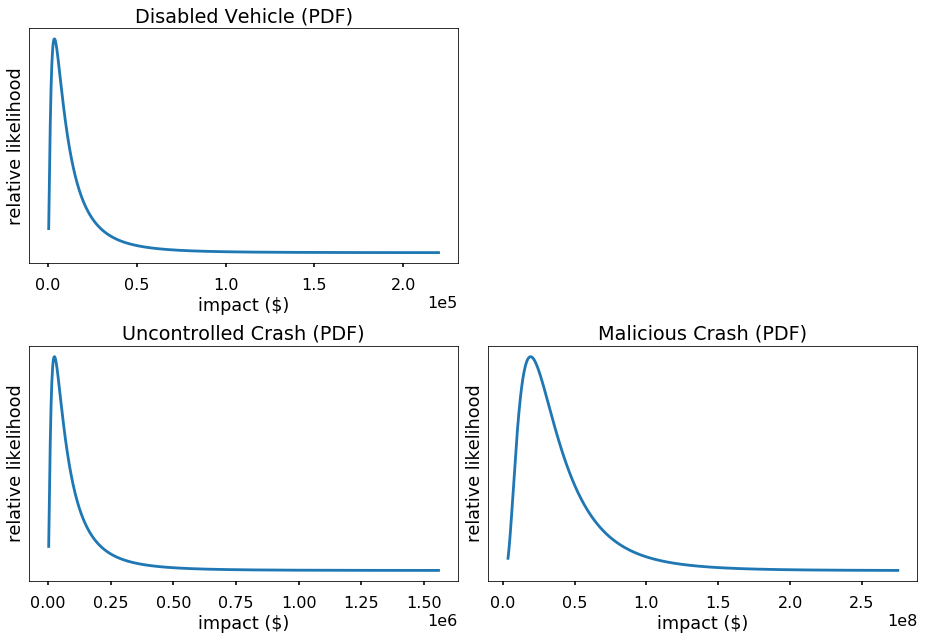
\includegraphics[width=\textwidth]{images/impacts.png}
    \caption{Impact probability density functions}
    \label{figure:impacts}
\end{figure}

Table \ref{table:results} presents a summary of threat sources, threat events, systems, controls, impacts, likelihoods, and risks. None of the threat sources, threat events, systems, controls, impacts, likelihoods, or risks are meant to be exhaustive. They merely provide a sample of different situations and how these differences respond to the risk assessment framework. This assessment considers twenty-four threat events:

\begin{enumerate}
\item Attacker gains access to teleoperation computer via outdated software on teleoperation computer: In this attack, an attacker is able to run malicious code on a teleoperation computer because of outdated software on the computer. Examples of outdated software are missing operating system patches or missing application patches. The malicious code could be downloaded by a user of the computer, or executed via the network. Controls against this attack include vulnerability management programs and remote operation protections. The likelihood of this attack is assumed to be once every ten years based on historical data and the impact is an intentional crash of a teleoperated vehicle.
\item Attacker gains access to teleoperation network via VPN: In this attack, an attacker gains remote access to a teleoperation facility via a VPN connection. Examples include weak VPN passwords and compromised accounts. This event is similar to the third event above but targets the teleoperation network instead of the vehicle network. Controls agains this attack include two-factor authentication and remote operation protections. The likelihood of this attack is assumed to be once every ten years based on historical data regarding password breaches and password reuse and the impact is an intentional crash of a teleoperated vehicle.
\item Attacker gains access to vehicle computer via outdated software: In this attack, an attacker is able to exploit a outdated software on a computer inside the vehicle. The attacker is then able to control the vehicle. Controls agains this attack include a vulnerability management program and remote operation protections. The likelihood of this attack is assumed to be once every ten years based on historical data of critical software vulnerabilities and the impact is an intentional crash of a vehicle.
\item Attacker gains access to vehicle via malware on teloperation computer: In this attack, an attacker is able to install malicious software on the teleoperation computer and then use this software to control the vehicle. Examples include a user who is tricked into installing malware or a malware that spreads across the network. Controls against this attack include anti-malware software and remote operation protections. The likelihood of this attack is assumed to be once every one hundred years and the impact is an intentional crash of a teleoperated vehicle.
\item Attacker gains access to vehicle via malware on vehicle computer: In this attack, an attacker is able to install malicious software on the a computer inside the vehicle and then use this software to control the vehicle. Examples include an attacker with physical access to the vehicle or a malware that spreads across the network. This event is similar to the one above except the malware is on a computer in the vehicle instead of a teleoperation computer. Controls against this attack include anti-malware software and remote operation protections. The likelihood of this attack is assumed to be once every one hundred years and the impact is an intentional crash of a vehicle.
\item Attacker gains access to vehicle wireless network: In this attack, an attacker is able to access a wireless network on the vehicle that is connected to the control system of the vehicle. This assessment does not consider any controls against this event but considers disabling the wireless network which eliminates the risk. The likelihood of this attack is assumed to be once every one hundred years and the impact is an intentional crash of a vehicle.
\item Attacker gains physical access to teleoperation computer: In this attack, an attacker gains physical access to a teleoperation computer and is able to use the computer to control a vehicle. Examples include breaking and entering or social engineering attacks. Controls against this attack include physical security controls at teleoperation facilities and remote operation protections. The likelihood of this attack is assumed to be once every one hundred years and the impact is an intentional crash of a teleoperated vehicle.
\item Attacker gains physical access to vehicle network: In this event, an attacker is able to physically connect to the vehicle network and control the vehicle. Controls against this attack include improving the physical security of the vehicles. The likelihood of this event is assumed to be once every one hundred years and the impact is an intentional crash of a vehicle.
\item Attacker gains remote access to vehicle network by exploiting software bug on WAN networking equipment:  In this attack, an attacker is able to exploit a software bug on the network equipment inside an autonomous vehicle. The attacker is then able to access the vehicle's network and control the vehicle. Controls against this attack include a vulnerability management program and remote operation protections. The likelihood of this attack is assumed to be once every one hundred years based on historical data and the impact is an intentional crash of a vehicle.
\item Attacker gains remote access to vehicle network via VPN: In this attack, an attacker gains remote access to an autonomous vehicle's network via a diagnostic VPN connection. Examples include weak VPN passwords and compromised accounts. Controls against this attack include two-factor authentication and remote operation protections. The likelihood of this attack is assumed to be once every ten years based on historical data regarding password breaches and password reuse and the impact is an intentional crash of a vehicle.
\item Attacker is hired as teleoperation driver: In this attack, an attacker is able to gain employment as a teleoperation driver. Controls against  this attack include background checks for teleoperation drivers. The likelihood of this attack is assumed to be once every one hundred years and the impact is an intentional crash of a vehicle.
\item Attacker jams radar signals: In this attack, an attacker is able to disrupt the radar signals from the autonomous vehicle and cause it to enter a fail-safe mode. This assessment does not consider any controls against this event. The likelihood of this attack is assumed to be once every one hundred years and the impact is a disabled vehicle.
\item Attacker spoofs radar signals: In this attack, an attacker manipulates the radar sensors of the autonomous such that surrounding cars are no longer detected. This assessment does not consider any controls against this event. The likelihood of this attack is assumed to be once every ten years and the impact is an accidental crash of a vehicle.
\item Denial of service attack against cellular network: In this event, an attacker disrupts the cellular network connection used for teleoperation of the vehicle. Examples of this attack include cellular blocking devices. This assessment does not consider any controls against this event. The likelihood of this event is assumed to be once every ten years and the impact is a disabled vehicle.
\item Theft of a teleoperation computer: In this event, a thief steals a computer from a teleoperation facility. Controls against this event include improving the physical security of the teleoperation facilities. The likelihood of this event is assumed to be once every ten years and the impact is a disabled vehicle.
\item Theft of a vehicle component: In this event, a thief steals a component from the vehicle. Examples include stealing a sensor or a computer. Controls against this event include improving the physical security of the vehicles. The likelihood of this event is assumed to be once every ten years and the impact is a disabled vehicle.
\item Bumps dislodge vehicle computers: In this event, a substantial bump in the road dislodges a computer in the vehicle. Examples include a cable coming lose, a computer resetting, or a computer failure. This assessment does not consider any controls against this event. The likelihood of this event is assumed to be once every year and the impact is an accidental crash of a vehicle.
\item Fire in the teleoperation facility: In this event, a fire starts in a teleoperation facility while a vehicle is being teleoperated. Examples include office fires. Controls against this event include a redundant teleoperation facility that can take over during a fire. The likelihood of this event is assumed to be once every one hundred years and the impact is an accidental crash of a vehicle.
\item Fire in the vehicle: In this event, a fire starts in the vehicle that destroys the control system. Examples include a passenger accidentally starting a fire or a vehicle component overheating and starting a fire. This assessment does not consider any controls against this event. The likelihood of this event is assumed to be once every ten years and the impact is an accidental crash of a vehicle.
\item Hardware failure of a teleoperation system: In this event, a critical hardware system in the teleoperation facility fails. Examples include a computer failure or power failure. Controls against this event include a redundant teleoperation facility that can take over during a failure. The likelihood of this event is assumed to be once every ten years and the impact is an accidental crash of a vehicle.
\item Hardware failure of a vehicle system: In this event, a critical hardware system in the vehicle fails. Examples include a computer failure, motor failure, or cable failure. This assessment does not consider any controls against this event. The likelihood of this event is assumed to be once every ten years and the impact is an accidental crash of a vehicle.
\item Rain/snow/fog disrupts sensors: In this event, weather events such as rain, snow or fog disrupts sensors on the vehicle. Examples include heavy rains obscuring a camera or snow obscuring a lidar sensor. This assessment does not consider any controls against this event. The likelihood of this event is assumed to be once every ten years and the impact is an accidental crash of a vehicle.
\item Vehicle crash dislodges sensors: In this event, an undetected vehicle crash physically moves a sensor from its calibrated position. Examples include a sideswipe crash that dislodges a side-mounted sensor. This assessment does not consider any controls against this event. The likelihood of this event is assumed to be once every year and the impact is an accidental crash of a vehicle.
\item Weather impacts cellular network: In this event, a weather event (rain, snow, etc.) reduces the ability of the cellular network to provide sufficient bandwidth for teleoperation. This assessment does not consider any controls against this event. The likelihood of this event is assumed to be two hundred times per year and the impact is a disabled vehicle.
\end{enumerate}

\begin{landscape}
\begin{longtable}{l | p{5cm} | p{4.5cm} | p{4.5cm} | p{1.75cm} | p{1.5cm} | p{1cm}}
   Threat Source &                                                                                             Threat Event &                                                                        System &                                                                                              Controls &  Impact (\$) (mean) &  Likelihood (mean) &  Risk (mean) \\
\hline
 Adversarial &  Attacker gains access to teleoperation computer via outdated software on teleoperation computer &  Teleoperation Facilities / Computer &  [Vulnerability management program, Autonomous system protections for remote operations] &  40398367 & 0.10 &  403 \\
 Adversarial &  Attacker gains access to teleoperation network via vpn &  Teleoperation Facilities / WAN networking equipment &  [Two-factor authentication, Autonomous system protections for remote operations] &  40398367 & 0.10 &  4039 \\
 Adversarial &  Attacker gains access to vehicle computer via outdated software &  Autonomous Vehicle / Computers &  [Vulnerability management program, Autonomous system protections for remote operations] &  40398367 & 0.10 &  403 \\
 Adversarial &  Attacker gains access to vehicle via malware on teloperation computer &  Teleoperation Facilities / Computer &  [Anti-malware software, Autonomous system protections for remote operations] &  40398367 & 0.01 &  403 \\
 Adversarial &  Attacker gains access to vehicle via malware on vehicle computer &  Autonomous Vehicle / Computers &  [Anti-malware software, Autonomous system protections for remote operations] &  40398367 & 0.01 &  403 \\
 Adversarial &  Attacker gains access to vehicle wireless network &  Autonomous Vehicle / Local Area Networks / WiFi &  [Disable WiFi] &  40398367 & 0.01 &  0 \\
 Adversarial &  Attacker gains physical access to teleoperation computer &  Teleoperation Facilities / Computer &  [Physical security at teleoperation facilities, Autonomous system protections for remote operations] &  40398367 & 0.01 &  403 \\
 Adversarial &  Attacker gains physical access to vehicle network &  Autonomous Vehicle / Local Area Networks &  [Physical security of vehicles] &  40398367 & 0.01 &  40398 \\
 Adversarial &  Attacker gains remote access to vehicle network by exploiting software bug on WAN networking equiptment &  Autonomous Vehicle / WAN networking equipment &  [Vulnerability management program, Autonomous system protections for remote operations] &  40398367 & 0.01 &  40 \\
 Adversarial &  Attacker gains remote access to vehicle network via vpn &  Autonomous Vehicle / WAN networking equipment &  [Two-factor authentication, Autonomous system protections for remote operations] &  40398367 & 0.10 &  4039 \\
 Adversarial &  Attacker is hired as teleoperation driver. &  People &  [Background checks for drivers] &  40398367 & 0.01 &  4039 \\
 Adversarial &  Attacker jams radar signals &  Autonomous Vehicle / Sensors / Radar &  [] &  16487 & 0.01 &  164 \\
 Adversarial &  Attacker spoofs radar signals &  Autonomous Vehicle / Sensors / Radar &  [] &  116779 & 0.10 &  11677 \\
 Adversarial &  Denial of service attack against cellular network &  Wide Area Networks / Cellular network &  [] &  16487 & 0.10 &  1648 \\
 Adversarial &  Theft of a teleoperation computer &  Teleoperation Facilities / Computer &  [Physical security at teleoperation facilities] &  16487 & 0.10 &  164 \\
 Adversarial &  Theft of a vehicle component &  Autonomous Vehicle &  [Physical security of vehicles] &  16487 & 0.10 &  164 \\
 Non-adversarial &  Bumps dislodge vehicle computers &  Autonomous Vehicle / Computers &  [] &  116779 & 1.00 &  116779 \\
 Non-adversarial &  Fire in the teleoperation facility &  Autonomous Vehicle &  [Redundant teleoperation facility] &  116779 & 0.01 &  11 \\
 Non-adversarial &  Fire in the vehicle &  Autonomous Vehicle &  [] &  116779 & 0.10 &  11677 \\
 Non-adversarial &  Hardware failure of a teleoperation system &  Teleoperation Facilities &  [Redundant teleoperation facility] &  116779 & 0.10 &  116 \\
 Non-adversarial &  Hardware failure of a vehicle system &  Autonomous Vehicle &  [] &  116779 & 0.10 &  11677 \\
 Non-adversarial &  Rain/snow/fog disrupts sensors &  Autonomous Vehicle / Sensors &  [] &  116779 & 0.10 &  11677 \\
 Non-adversarial &  Vehicle crash dislodges sensors &  Autonomous Vehicle / Sensors &  [] &  116779 & 1.00 &  116779 \\
 Non-adversarial &  Weather impacts cellular network &  Wide Area Networks / Cellular network &  [] &  16487 & 200.00 &  3297442 \\
     \caption{Results}
    \label{table:results}
    \end{longtable}
\end{landscape}

% Another consideration is the average cost of a malware attack in 2017 was \$2,400,000 \citep{richards_2017_2017}. And the average cost of a data breach was \$ 3,620,000 \citep{ponemon_institute_llc_2017_2017}.

Figure \ref{figure:ael} shows the annual expected loss for this autonomous vehicle system given no controls (upper blue line) and optimal controls (lower green line). The no controls situation is determined by running the Monte Carlo simulation described in section \ref{subsubsection:determine_risk} with no controls implemented. The optimal controls situation is determined by running the Monte Carlo simulation with optimal controls enabled. Determining optimal controls is discussed below.

This figure shows the probability of a given loss in a given year and the impact security controls can have on reducing losses. The annual expected loss does not include the cost of controls. This figure aids the control selection process by showing the best and worst case scenarios. For example, given a set of controls, it is possible to determine the probability of a loss over a certain amount. If this loss is acceptable, the controls can be implemented and the system can be put in service. If this loss is unacceptable, additional controls (or other methods of managing risk) are necessary. Even in the situation of optimal controls, a considerable loss is expected each year. This is because there are several risks such as "Weather impacts cellular network" that remain unmitigated.

\begin{figure}[h] \centering
    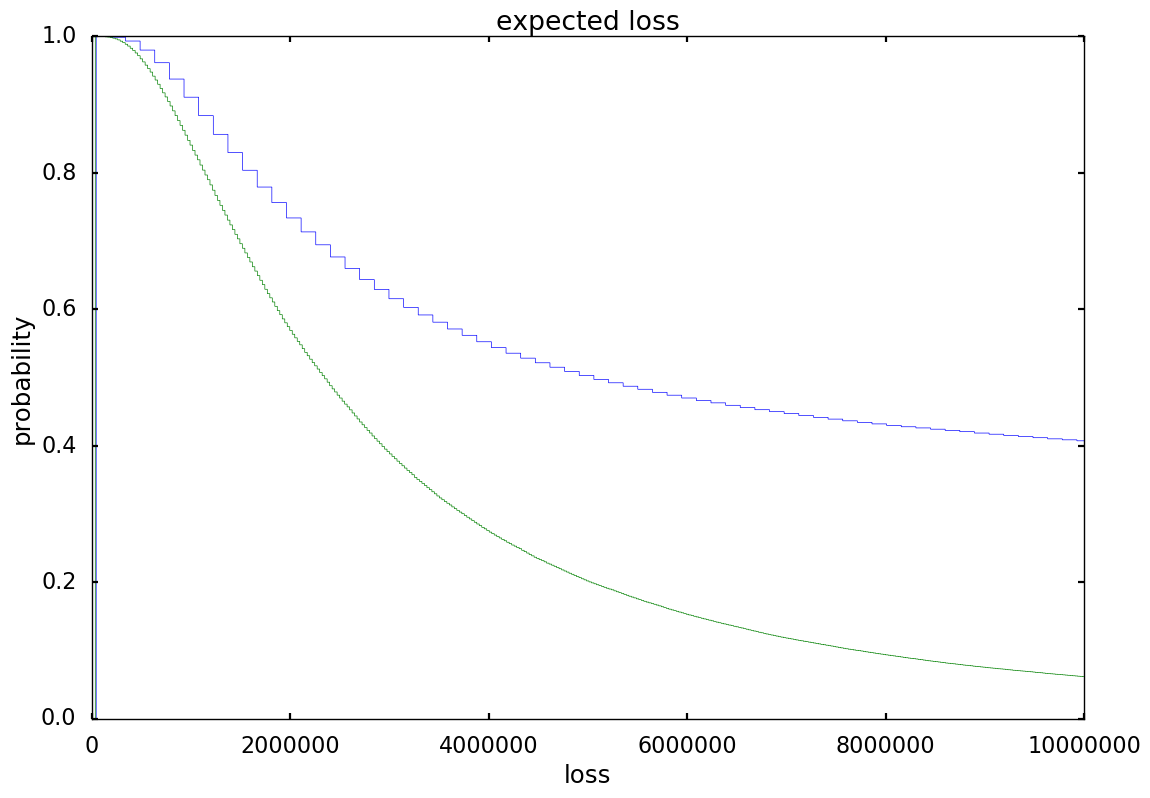
\includegraphics[width=\textwidth]{images/ael.png}
    \caption{Annual expected loss (\$/year); upper blue line is with no controls, lower green line is with optimal controls}
    \label{figure:ael}
\end{figure}


\subsection{Optimization of Controls}
The controls used in this assessment (Table \ref{table:optimal_controls}) represent a sample of possible controls that could protect an autonomous vehicle system. A real such system would likely have hundreds, if not thousands, of controls. The costs and reduction factors are samples used to study how the risk assessment framework responds to differences.

The results of optimizing security controls are shown in Table \ref{table:optimal_controls} and Figure \ref{figure:riskvscost}. The table show the cost and reduction factor as well as if the control is implemented in the optimal system. More effective controls that mitigate multiple risks (such as "Autonomous system protections for remote operations") are much more valuable than targeted controls that only protect against specific threat events (such as "Anti-malware software"). Additionally, adding a safety driver control at the cost of an average professional proves far more expensive than equivalent security controls for reducing risk. Interestingly, a sensitivity analysis performed by changing the costs of controls according to a log normal distribution while continually optimizing these controls always resulted in the same set of optimal controls. This is probably because the differences in costs and reduction factors are relatively large between different controls.

\begin{table}[h]\begin{center}
\begin{tabular}{l | r | r | l}
{}  &    Cost (\$) & Reduction factor  & Implemented  \\
\hline
Vulnerability management program                    &  100000 &  0.01& False  \\
Anti-malware software                               &  10000 & 0.10  & False \\
Two-factor authentication                           &  50000 & 0.10  & True \\
Disable WiFi                                        &  1000 & 0.00  &True  \\
Physical security at teleoperation facilities       &  10000 &0.10   & False \\
Physical security of vehicles                       &  100000 &0.10   &  True\\
Redundant teleoperation facility                    &  100000 &  0.01 & False \\
Autonomous system protections for remote operations &  500000 &0.01   & True \\
Background checks for drivers                       &  10000 & 0.01  & True \\
\end{tabular}
    \caption{Optimal controls}
    \label{table:optimal_controls}
\end{center} \end{table}

Figure \ref{figure:riskvscost} shows one point representing the residual risk and cost for each control combinations. For example, when few controls are implemented as on the left side of the graph, the control cost is low, but the residual risk is high. As the control cost increases, the residual risk tends to increase. The point of optimal controls show in Table \ref{table:optimal_controls}, defined as the point closest to the origin, is colored red. It is also interesting to see how control combinations cluster and follow patterns around the graph because enabling or disabling one control shifts the group.
 
\begin{figure}[h] \centering
    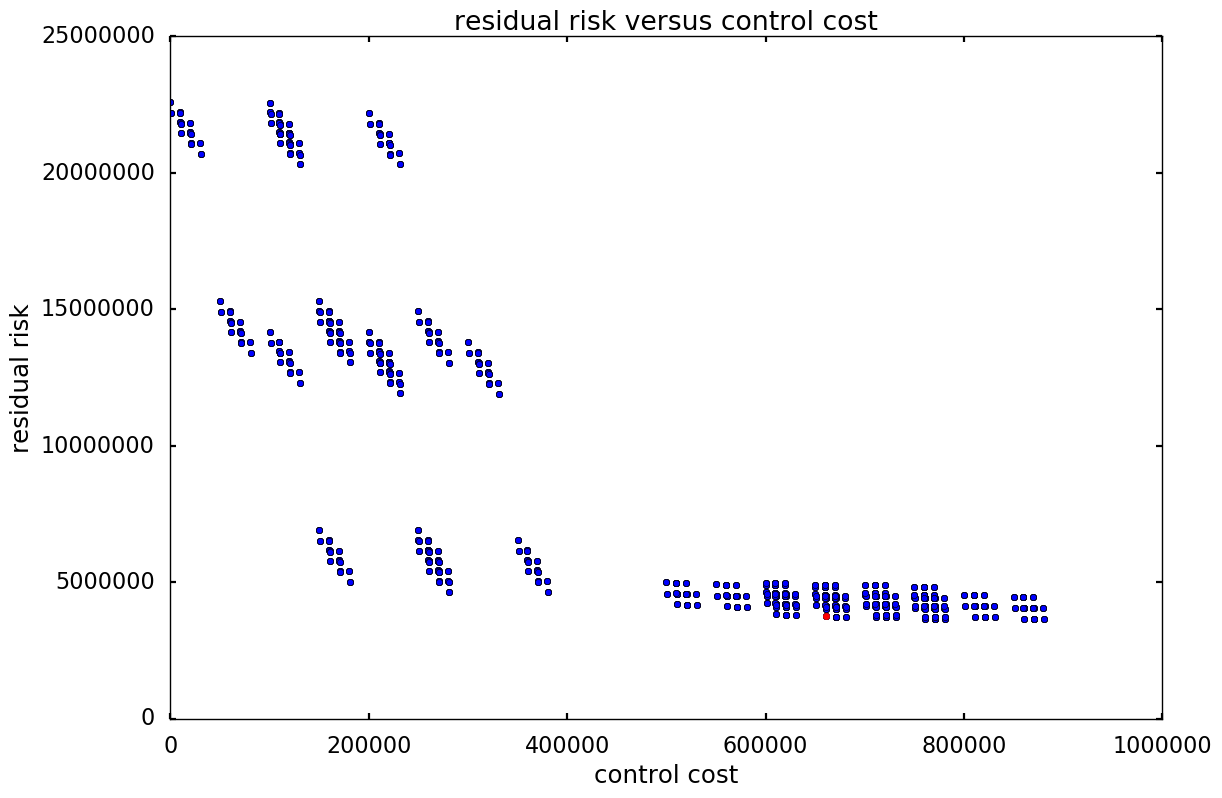
\includegraphics[width=\textwidth]{images/riskvscost.png}
    \caption{Residual risk versus control cost (\$); optimal controls are red}
    \label{figure:riskvscost}
\end{figure}


\newpage
\section{Discussion}

\begin{mdframed}
    \emph{What they had in common was mainly love of excellence and programming. They wanted to make their programs that they used be as good as they could. They also wanted to make them do neat things. They wanted to be able to do something in a more exciting way than anyone believed possible and show "Look how wonderful this is. I bet you didn't believe this could be done."} \\ -- Richard \cite{stallman_hackers_1985}
\end{mdframed}

\noindent Most of the attacks mentioned in the introduction target the lateral (steering) and longitudinal (acceleration and braking) control systems that can obviously cause a vehicle to crash. However, other attacks against headlights could compromise computer vision systems and also cause vehicles to crash or attacks against entertainment systems could damage passengers' hearing. Specialized vehicles including buses, taxis, and trucks also have unique attack vectors that must be considered for their threat models. For examples, taxis often have a tablet for passengers to interact with, and trucks do not have passengers.

While this thesis focused on autonomous road vehicles, several other autonomous vehicle types are currently under development or in production including unmanned aerial vehicles, autonomous ships, and small autonomous delivery robots. These vehicles bear similar risks and consequently deserve study.

Similar to when other industries transitioned to electronic records, the legal structure around autonomous vehicles is not well defined. For example, California Penal Code 502 defines an injury as "any alteration, deletion, damage, or destruction of a computer system, computer network, computer program, or data caused by the access, or the denial of access to legitimate users of a computer system, network, or program" \citep{waldron_california_2015}. However, this ignores cases where an attacker uses a computer to cause physical injury to property or persons. Likewise, the issue who is liable for the damage caused by a hacked autonomous vehicle has not been determined. The United States Congress appears to be aware of autonomous vehicle security, but has failed to pass legislation addressing the issue \citep{latta_self_2017, thune_av_2017}.

In addition to legal regulations, autonomous vehicle industry groups are still in their infancy in regards to security. In 2014, the Alliance of Automobile Manufacturers, Inc. and the Association of Global Automakers, Inc. formed the Automotive Information Sharing \& Analysis Center (Auto-ISAC) upon recommendation of the National Highway Traffic Safety Administration \citep{bainwol_letter_2014, beuse_docket_2014}. The purpose of this organization, similar to other ISAC organizations in other industries, is to develop and share security information such as their Automotive Cybersecurity Best Practices \citep{automotive_information_sharing_and_analysis_center_auto-isac_automotive_}. To date they have released best practices guides for Incident Response and Third Party Collaboration and Engagement.

There are other automotive security industry groups predating modern autonomous vehicles. The Motor Industry Software Reliability Association (MISRA) released versions of C and C++ designed for automotive use. Also, formal methods provide a way to validate safety in safety-critical software. However, it appears many vehicle manufacturers neglect to use these methods and often blame drivers for what may be software faults \citep{koopman_practical_2018}. It will be interesting to see how this behavior changes when drivers are not be there to blame. While this thesis limited the focus to security events, vehicle safety and security are fundamentally connected. Automotive safety practices such as the failure mode and effects analysis (FMEA) are similar to security risk management. Autonomous vehicle systems should explore combining safety and security efforts when practicable.

Another issue is support for security updates when new vulnerabilities are discovered. GM took 5 years to fix a security flaw in their 2009 Chevrolet Impala \citep{greenberg_gm_2015}. Some manufacturers, including GM, have technology to provide over-the-air updates \citep{2007-01-3523, 2014-01-0256, lewis_over--air_2016, alrabady_secure_2011}, but these mechanisms also present a security risk themselves. Also, for how long do manufacturers have to provide security updates? What about software written by third parties? And, do owners have any rights to write their own security software?

Vehicle systems have unique characteristics that must be considered during the risk management process. The Controller Area Network (CAN bus) is an in-vehicle communication network created by BOSCH and first implemented in the 1988 BMW 8-Series \citep{international_organization_for_standardization_iso_2015}. It allows open communication between electronic control units (ECUs) and can be exploited via denial of service attacks, spoofed messages, and sniffed messages \citep{kleberger_security_2011, miller_adventures_2014, miller_advanced_2016, miller_can_2016, smith_car_2016}. Several researchers have proposed intrusion detections systems (IDS) \citep{larson_approach_2008, muter_entropy-based_2011, boudguiga_simple_2016, song_intrusion_2016, kang_intrusion_2016, cho_fingerprinting_2016, daxin_tian_intrusion_2018, spicer_intrusion_2018}, or encryption systems \citep{bruton_securing_2014, wei_authenticated_2016, mukund_security_2015} for the CAN bus. Similarly, some autonomous vehicles use the Robot Operating System (ROS) which bears many similarities to CAN: ROS is an open network and any node (analogous to an ECU) can openly communicate with other nodes. Several projects aim to add security features to ROS such as authentication and encryption \citep{dieber_security_2017, breiling_secure_2017}.

NIST Special Publication 800-30 notes that quantitative assessments often require more time and effort than qualitative assessments \citep{national_institute_of_standards_and_technology_nist_2012}. However, the results shown in this thesis would not be possible within a qualitative framework. One area of quantitative assessments that could be greatly improved is the determination of likelihoods and impacts. Further research into methods for robustly gathering this data is welcome. For now, most of this data is based on educated guesses of experienced professionals. Also, because autonomous vehicles are relatively new and large-scale deployments do not yet exist, much of this data is simply unavailable. In the era of big data, rare events prove problematic for quantitive risk management frameworks.

% VANETs (Vehicular Ad-hoc NETworks) should "achieve considerable penetration only around 2014" \citep{raya_securing_2007}

\newpage
\section{Conclusion}

\begin{mdframed}
    \emph{No fim, tudo d\'{a} certo. Se n\~{a}o deu, ainda n\~{a}o chegou ao fim. \\ (In the end, everything will be ok. If it's not ok, it's not yet the end.)} -- Fernando Sabino
\end{mdframed}

\noindent Autonomous vehicles have arrived. Qualitative risk management frameworks allow the companies architecting these autonomous vehicle systems to measure their security risks, choose the most appropriate security controls, and assure a level of safety. Existing information security approaches are well suited to securing the robotic systems that control autonomous vehicles. The transportation industry can learn from past security mistakes in other industries.

Traditional, qualitative frameworks have several shortcomings including an inability to mathematically sum, compare, and interpret risks. Quantitative frameworks, while requiring more data, help risk management programs overcome these limitations. Annual expected loss curves to show the probability of different loss levels given different security controls. Optimization techniques to select the best security controls for a system. Quantitative frameworks communicate risk clearly in monetary units instead of "high, medium, and low" risk levels.

Similar to the safety ratings of passenger cars, qualitative risk management provides a method for impartial evaluation of the security risks present in an autonomous vehicle system. Quantitative risk management methods can also be applied to other areas of transportation such as safety modeling, environmental impact modeling, traffic management, and cost-benefit analysis. Also, these techniques can be expanded to cover other modes including active transportation, freight, and private public partnerships.

As Heidi King, Deputy Administrator of the National Highway Traffic Safety Administration said "we should together build and support a cyber security risk management culture for the automotive industry that can serve as a role model to others. Our national automotive safety depends on it" \citep{king_remarks_2018}.


\newpage
\section{Appendix I: MIL-STD-882E Risk Tables}

\begin{table}[h]
    \begin{tabularx}{\linewidth}{c | c | X}
        Description & Severity & Mishap Result Criteria \\ \hline
        Catastrophic & 1 & Could result in one or more of the following: death, permanent total disability, irreversible significant environmental impact, or monetary loss equal to or exceeding \$10M. \\
        Critical & 2 & Could result in one or more of the following: permanent partial disability, injuries or occupational illness that may result in hospitalization of at least three personnel, reversible significant environmental impact, or monetary loss equal to or exceeding \$1M but less than \$10M. \\
        Marginal & 3 & Could result in one or more of the following: injury or occupational illness resulting in one or more lost work day(s), reversible moderate environmental impact, or monetary loss equal to or exceeding \$100K but less than \$1M. \\
        Negligible & 4 & Could result in one or more of the following: injury or occupational illness not resulting in a lost work day, minimal environmental impact, or monetary loss less than \$100K. \\
    \caption{MIL-STD-882E Severity Rankings \citep{department_of_defense_mil-std-882e_2012}}
    \end{tabularx}
    \label{department_of_defense_mil-std-882e_2012_severity_rankings}
\end{table}

\begin{table}[h]
    \begin{tabularx}{\linewidth}{c | c | X | X}
        Description & Level & Specific Individual Item & Fleet or Inventory \\ \hline
        Frequent & A & Likely to occur often in the life of an item. & Continuously experienced \\
        Probable & B & Will occur several times in the life of an item. & Will occur frequently. \\
        Occasional & C & Likely to occur sometime in the life of an item. & Will occur several times. \\
        Remote & D & Unlikely, but possible to occur in the life of an item. & Unlikely, but can reasonably be expected to occur. \\
        Improbable & E & So unlikely, it can be assumed occurrence may not be experienced in the life of an item. & Unlikely to occur, but possible. \\
        Eliminated & F & Incapable of occurrence. This level is used when potential hazards are identified and later elimi nated. & Incapable of occurrence. This level is used when potential hazards are identified and later eliminated \\
    \caption{MIL-STD-882E Probability Levels \citep{department_of_defense_mil-std-882e_2012}}
    \end{tabularx}
    \label{department_of_defense_mil-std-882e_2012_probability_levels}
\end{table}

\begin{table}[p]
    \begin{tabularx}{\linewidth}{ X | X | X | X | X}
        & Catastrophic (1) & Critical (2) & Marginal (3) & Negligible (4) \\ \hline
        Frequent (A) & \textcolor{red}{High} & \textcolor{red}{High} & \textcolor{orange}{Serious} & \textcolor{yellow}{Medium} \\
        Probable (B) & \textcolor{red}{High} & \textcolor{red}{High} & \textcolor{orange}{Serious} & \textcolor{yellow}{Medium} \\
        Occasional (C) & \textcolor{red}{High} & \textcolor{orange}{Serious} & \textcolor{yellow}{Medium} & \textcolor{green}{Low} \\
        Remote (D) & \textcolor{orange}{Serious} & \textcolor{yellow}{Medium} & \textcolor{yellow}{Medium} & \textcolor{green}{Low} \\
        Improbable (E) & \textcolor{yellow}{Medium} & \textcolor{yellow}{Medium} & \textcolor{yellow}{Medium} & \textcolor{green}{Low} \\
        Eliminated (F) & \textcolor{blue}{Eliminated} & \textcolor{blue}{Eliminated} & \textcolor{blue}{Eliminated} & \textcolor{blue}{Eliminated} \\
    \caption{MIL-STD-882E Risk Matrix \citep{department_of_defense_mil-std-882e_2012}}
    \end{tabularx}
    \label{department_of_defense_mil-std-882e_2012_risk_matrix}
\end{table}

\newpage
\section{Appendix II: ASIL Risk Tables}

\begin{table}[h]
    \begin{tabularx}{\linewidth}{ c | X | X | X | X}
 & E1 & E2 & E3 & E4 \\ \hline
Duration & - & \textless 1\% of operating time & 1-10\% of operating time & \textgreater 10\% operating time \\
Frequency & Occur less than once a year & Situation that occurs a few times a year & Situation that occurs once a month & Situations that occur almost every drive \\
Examples & Driving downhill with engine off & Driving on unsecured steep slope & Slippery roads & Braking \\
    \caption{ASIL Probability/Exposure \citep{international_organization_for_standardization_iso_2011}}
    \end{tabularx}
    \label{international_organization_for_standardization_iso_2011_probability}
\end{table}

\begin{table}[h]
    \begin{tabularx}{\linewidth}{ c | X | X | X}
 & S1 & S2 & S3 \\ \hline
Description & Light and moderate injuries & Severe injuries, possibly life threatening, survival probable. & Life threatening injuries, survival uncertain, fatal injuries \\
Example & Collision with tree \textless 20 kpm & Collision with tree 20-40 kpm & Collision with tree \textgreater 40 kpm \\
    \caption{ASIL Severity \citep{international_organization_for_standardization_iso_2011}}
    \end{tabularx}
    \label{international_organization_for_standardization_iso_2011_severity}
\end{table}

\begin{table}[h]
    \begin{tabularx}{\linewidth}{ c | X | X | X}
 & C1 & C2 & C3 \\ \hline
Description & Simply controllable & Normally controllable & Difficult to control or uncontrollable \\
Definition & All drivers will be able to avoid it & 90\% of all drivers will be able to avoid it & 10\% of all drivers will be able to avoid it \\
Example & Starting a vehicle with locked steering & Stopping a vehicle in case of light failure & Loss of breaks \\
    \caption{ASIL Controllability \citep{international_organization_for_standardization_iso_2011}}
    \end{tabularx}
    \label{international_organization_for_standardization_iso_2011_controllability}
\end{table}

\newpage
\section{Appendix III: OWASP Risk Rating Methodology}
\begin{table}[h]\begin{center}
    \begin{tabularx}{\linewidth}{ X | X | X | X }
        Likelihood / Impact & Low & Medium & High \\ \hline
        High & \textcolor{orange}{Medium} & \textcolor{red}{High} & \textcolor{pink}{Critical} \\
        Medium & \textcolor{yellow}{Low} & \textcolor{orange}{Medium} & \textcolor{red}{High} \\
        Low & \textcolor{green}{Note} & \textcolor{yellow}{Low} & \textcolor{orange}{Medium} \\
    \caption{Overall risk severity \citep{open_web_application_security_project_owasp_2016}}
    \end{tabularx}
    \label{open_web_application_security_project_owasp_2016}
\end{center}\end{table}

\newpage
\section{Appendix IV: Security Control Identifiers}
\begin{figure}[h]
    \begin{itemize}
        \item{Access Control}
	\item{Audit and Accountability}
	\item{Awareness and Training}
	\item{Configuration Management}
	\item{Contingency Planning}
	\item{Identification and Authentication}
	\item{Incident Response}
	\item{Maintenance}
	\item{Media Protection}
	\item{Personnel Security}
	\item{Physical and Environmental Protection}
	\item{Planning}
	\item{Program Management}
	\item{Risk Assessment}
	\item{Security Assessment and Authorization}
	\item{System and Communications Protection}
	\item{System and Information Integrity}
	\item{System and Services Acquisition}
    \end{itemize}
    \caption{Security Control Identifiers \citep{national_institute_of_standards_and_technology_nist_2013}}
    \label{enumerate:national_institute_of_standards_and_technology_nist_2013}
\end{figure}

\newpage
\section{Appendix V: CIS Controls}
\begin{figure}[h]
    \begin{itemize}
    \item{Basic CIS Controls}
        \begin{enumerate}
        \item{Inventory and Control of Hardware Assets}
        \item{Inventory and Control of Software Assets}
        \item{Continuous Vulnerability Assessment and Remediation}
        \item{Controlled Use of Administrative Privileges}
        \item{Secure Configuration for Hardware and Software on Mobile Devices, Laptops, Workstations, and Servers}
        \item{Maintenance, Monitoring, and Analysis of Audit Logs}
        \end{enumerate}
    \item{Foundational CIS Controls}
        \begin{enumerate}
        \setcounter{enumi}{6}
        \item{Email and Web Browser Protections}
        \item{Malware Defenses}
        \item{Limitations and Control of Network Ports, Protocols, and Services}
        \item{Data Recovery Capabilities}
        \item{Secure Configurations for Network Devices, such as Firewalls, Routers, and Switches}
        \item{Boundary Defense}
        \item{Data Protection}
        \item{Controlled Access Based on the Need to Know}
        \item{Wireless Access Control}
        \item{Account Monitoring and Control}
        \end{enumerate}
    \item{Organizational CIS Controls}
        \begin{enumerate}
        \setcounter{enumi}{16}
        \item{Implement a Security Awareness and Training Program}
        \item{Application Software Security}
        \item{Incident Response and Management}
        \item{Penetration Tests and Red Team Exercises}
        \end{enumerate}
    \end{itemize}
    \caption{CIS Controls \citep{center_for_internet_security_cis_2018}}
    \label{enumerate:center_for_internet_security_cis_2018}
\end{figure}

\newpage
\section{Appendix VI: PCI Data Security Standard -- High Level Overview}
\begin{table}[h]
    \begin{tabularx}{\textwidth}{p{4.2cm} X}
        Control Objectives & PCI DSS Requirements\\
        \hline
        Build and Maintain a Secure Network and Systems & 1. Install and maintain a firewall configuration to protect cardholder data \\
            & 2. Do not use vendor-supplied defaults for system passwords and other security parameters \\
        Protect Cardholder Data & 3. Protect stored cardholder data \\
            & 4. Encrypt transmission of cardholder data across open, public networks \\
        Maintain a Vulnerability Management Program & 5. Protect all systems against malware and regularly update anti-virus software or programs \\
            & 6. Develop and maintain secure systems and applications \\
        Implement Strong Access Control Measures & 7. Restrict access to cardholder data by business need to know 8. Identify and authenticate access to system components \\
            & 9. Restrict physical access to cardholder data \\
        Regularly Monitor and Test Networks & 10. Track and monitor all access to network resources and cardholder data \\
            & 11. Regularly test security systems and processes \\
        Maintain an Information Security Policy & 12. Maintain a policy that addresses information security for all personnel \\
    \caption{PCI Data Security Standard -- High Level Overview \citep{pci_security_standards_council_payment_2016}}
    \end{tabularx}
    \label{table:pci_security_standards_council_payment_2016}
\end{table}

\newpage
\printglossaries

\newpage
\bibliographystyle{plainnat}
\bibliography{references}

\newpage
\section{Colophon}

\begin{mdframed}
    \emph{If I have seen further it is by standing on the shoulders of Giants.} -- Sir Isaac \cite{newton_letter_1675}
\end{mdframed}

\noindent This thesis was possible because of the dedication and generosoty of open source developers throughout the world. This thesis was written with TeXShop (Richard Koch) using the \LaTeX \ document preparation system (Leslie Lamport) which is based on \TeX \ (Donald E. Knuth). Diagrams were drawn with PGF/Ti\emph{k}Z (Till Tantau). References were managed with Zotero (Center for History and New Media at George Mason University) and exported to \hologo{BibTeX} (Oren Patashnik and Leslie Lamport). The original \LaTeX and \hologo{BibTeX} files along with this compiled PDF are available at \url{https://davidabailey.com/thesis}.


The quantitative risk assessment tool was written with Jupyter Lab (Fernando P\'{e}rez) in the Python programming language (Guido van Rossum) and uses numpy (Travis Oliphant) which is based on Numeric (Jim Hugunin) which is based on Jim Fulton's matrix object, pandas (Wes McKinney), matplotlib (John Hunter), and scipy (Travis Oliphant, Pearu Peterson, and Eric Jones). The Python code is available at \url{https://davidabailey.com/thesis}.


\end{document}